\chapter{Result discussion}
The main advantage of CFD analysis is its ability to calculate all flow parameters 
at every grid point in the domain studied, allowing for a very detailed description of the
flow. The present study can be classified into two main parts: Firstly, the
noncavitating flow and cavitating flow over the proposed NACA0012 hydrofoil, $\&$
secondly, the modeling and computations of unsteady cavitation shedding using k-$\omega$ sst turbulence model. In this
study, Cl and Cd are validated for a fixed cavitation number with different $\sigma$/{2$\alpha$} which is 
range from 2.86 to 7 are computed. The reason for choosing this range is because, in the reference\cite{Zhao2021}, it states 
the limitation of using  k-$\omega$ sst model at a higher angle of attack.
The lift and drag coefficient are computed as below:
\begin{equation}
{C_L}=\frac{L}{{\frac{1}{2}}{{\rho}_{\infty}}{{{U}^2}_{\infty}}{S_{ref}}}
\end{equation}
\begin{equation}
{C_D}=\frac{D}{{\frac{1}{2}}{{\rho}_{\infty}}{{{U}^2}_{\infty}}{S_{ref}}}
\end{equation}
where q=${{\frac{1}{2}}{{\rho}_{\infty}}{{{U}^2}_{\infty}}{S_{ref}}}$=1875 N.\\ 
The corresponding pressure coefficient is calculated by:
\begin{equation}
{C_p}=\frac{P-{P_{\infty}}}{{\frac{1}{2}}{{\rho}_{\infty}}{{{U}^2}_{\infty}}}
\end{equation}
\section{Non cavitating steady flow}
The computational duration was 1 s long to ensure that the cavitation flow was fully developed. Firstly, 
the non-cavitating steady flow was calculated to verify the performance of the grid. The unsteadiness was not trigged in the range of $\sigma$/{2$\alpha$}  
between 6 to 7 whose angle of attack $\alpha$ ranges from 3.2 to 3.8. The condition to occur cavitation was not respected 
in this range which means the local pressure was not well below the vapor pressure. The flow is attached to wall  and the detailed 
information of the flow field from the NACA0012 wet flow simulation result calculated by OpenFOAM is reliable while comparing the result 
with experimental data of the given range. Because of the steady flow, it is fine enough to show the result with the final 
time step which is shown below:\\
\begin{table}[h]
\centering
\begin{tabular}{|l|l|}
\hline
\rowcolor{gray!20} $\frac{\sigma}{2\alpha}$(radians)&$\alpha$(degree) \\ \hline
 2.86&8  \\ \hline
 3& 7.6 \\ \hline
 3.5&6.5  \\ \hline
 4& 5.7 \\ \hline
4.5 &5.0  \\ \hline
5 & 4.5 \\ \hline
 5.5&4.1  \\ \hline
 6& 3.8 \\ \hline
6.5 & 3.5 \\ \hline
 7& 3.2 \\ \hline
\end{tabular}
\caption{$\frac{\sigma}{2\alpha}$ and its corresponding $\alpha$}
\label{}
\end{table}
As can be seen from the figure(4.1$\&$4.2), there is a low-pressure area on the suction side of the hydrofoil 
and a high-pressure area on the pressure side. There is a progressive increase in the local velocity 
with a decrease in local pressure over the suction side of the hydrofoil to the 
increase of angle of attack. 

\begin{figure}[H]
    \centering
    \subfloat[$3.2^{\circ}$]{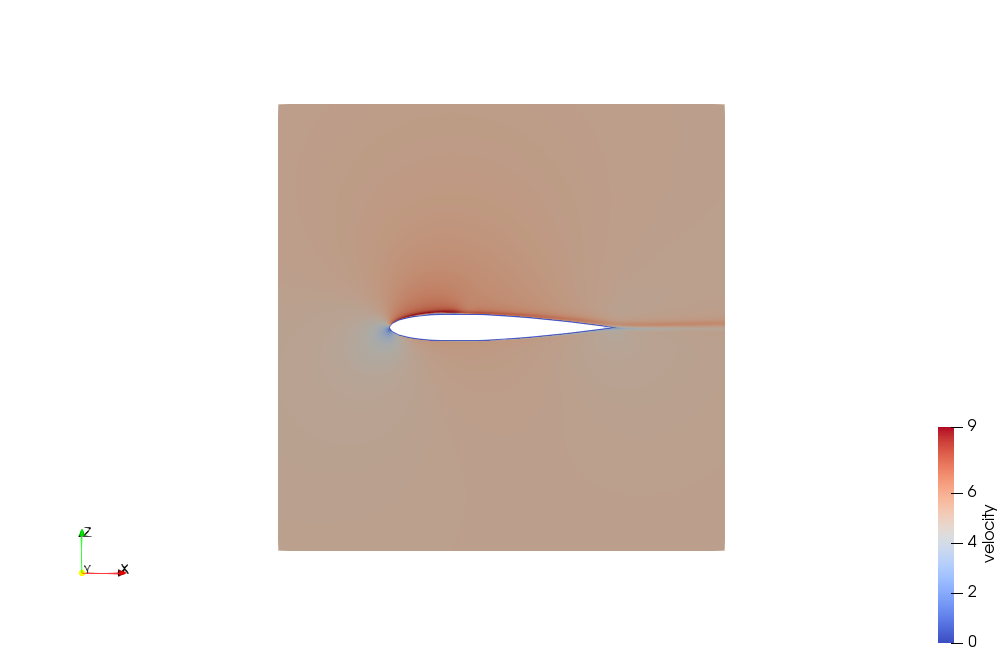
\includegraphics[width=0.3\textwidth]{AOA3.2p/AOA3.2t1v}}
    \qquad
  \subfloat[$3.5^{\circ}$]{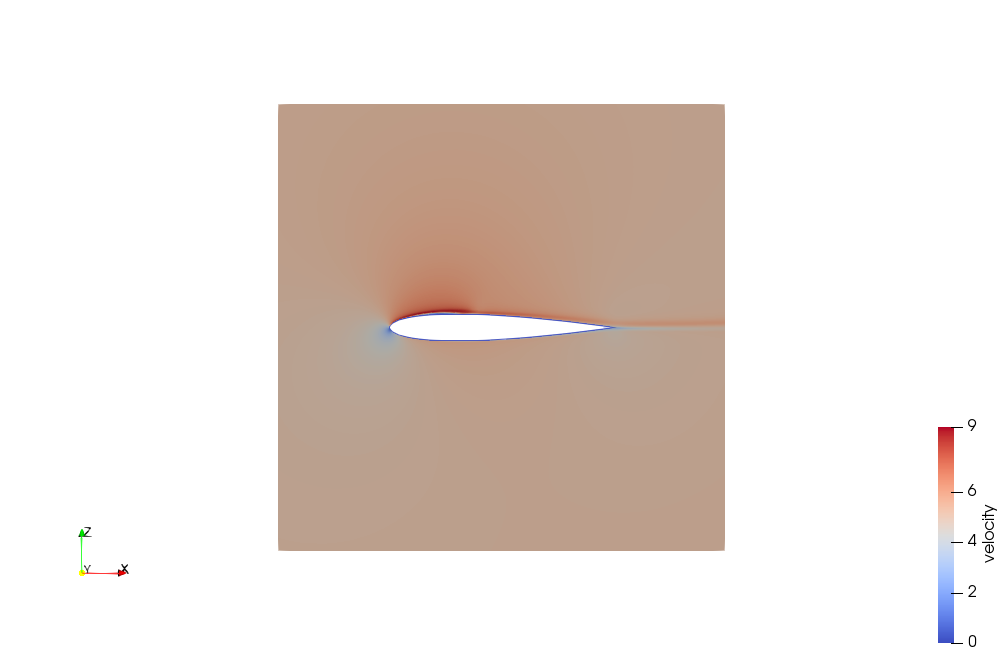
\includegraphics[width=0.3\textwidth]{AOA3.5p/AOA3.5t1v}}
   \qquad
  \subfloat[$3.8^{\circ}$]{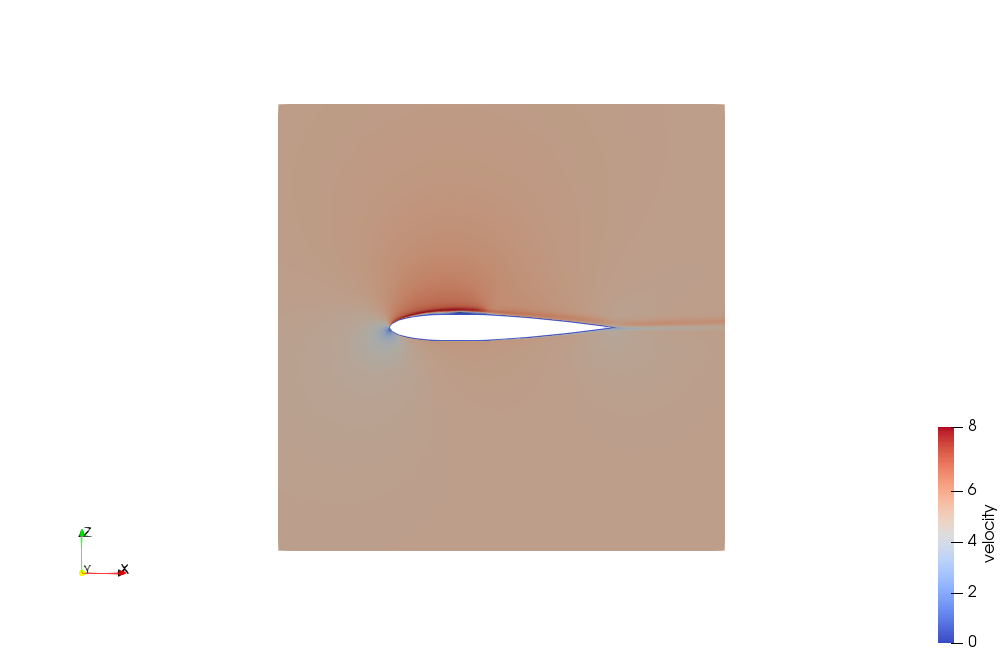
\includegraphics[width=0.3\textwidth]{AOA3.8p/AOA3.8t1v}}
      \caption{Change in velocity over a NACA0012, non cavitating flow}
    \label{fig:fig16}
\end{figure}
 \begin{figure}[H]
    \centering
    \subfloat[$3.2^{\circ}$]{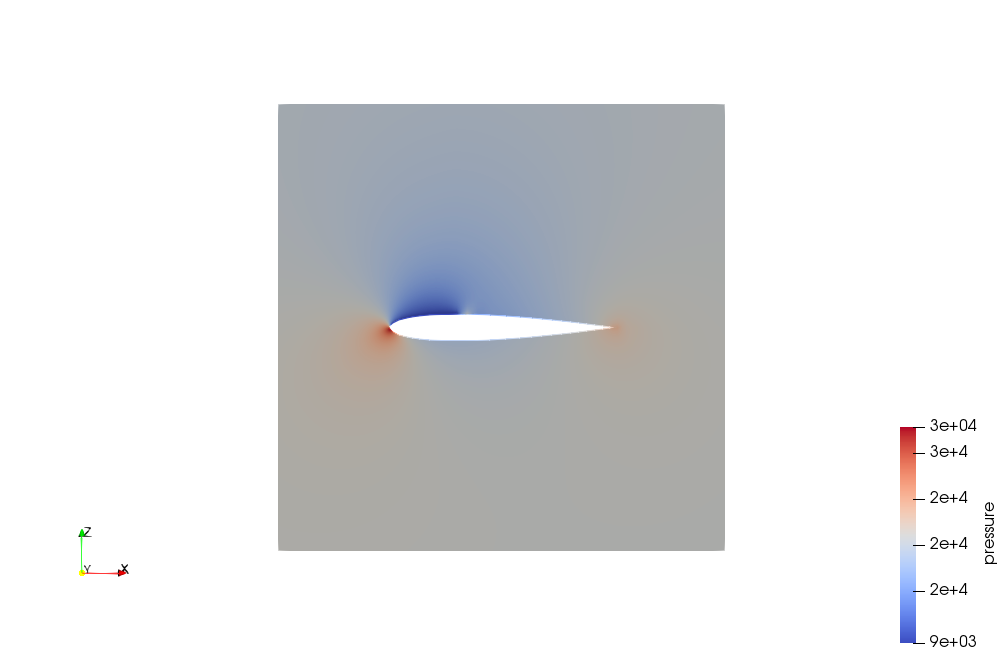
\includegraphics[width=0.3\textwidth]{AOA3.2p/AOA3.2t1p}}
    \qquad
  \subfloat[$3.5^{\circ}$]{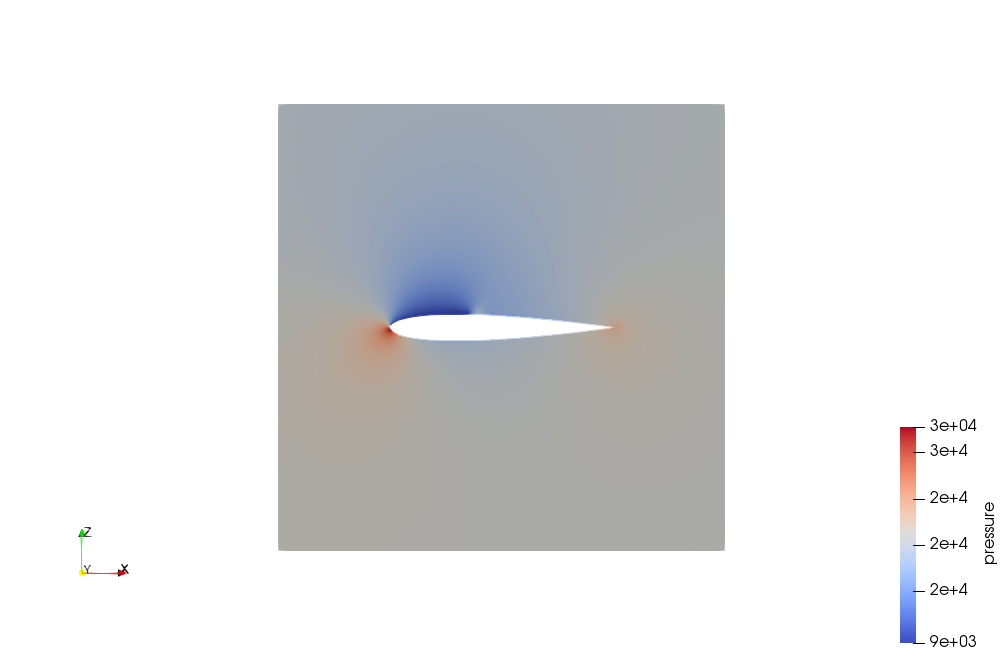
\includegraphics[width=0.3\textwidth]{AOA3.5p/AOA3.5t1p}}
   \qquad
  \subfloat[$3.8^{\circ}$]{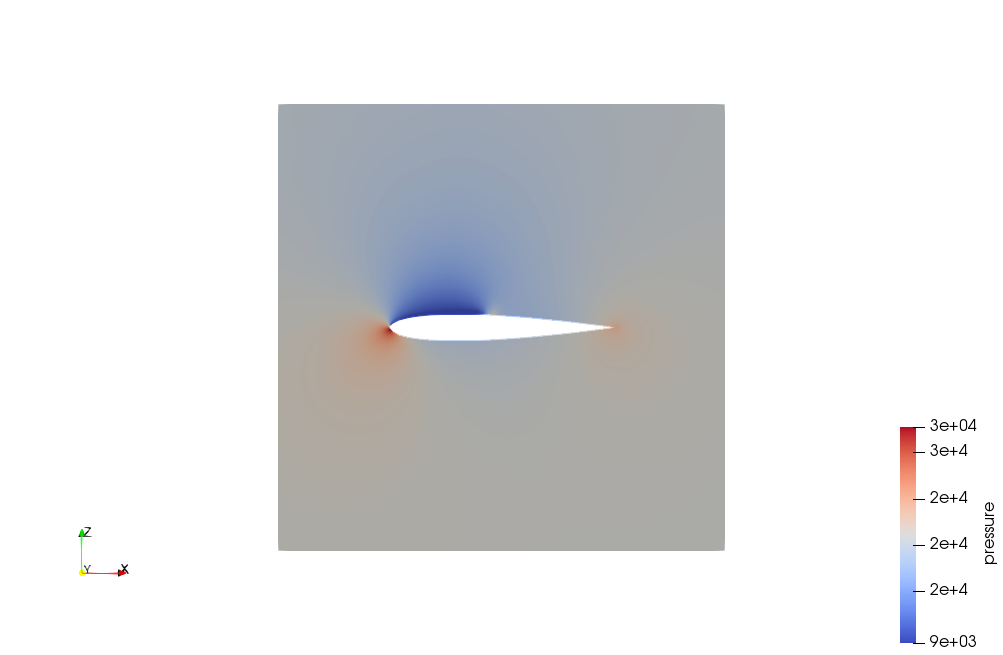
\includegraphics[width=0.3\textwidth]{AOA3.8p/AOA3.8t1p}}
      \caption{Change in pressure over a NACA0012, non cavitating flow}
    \label{fig:fig16}
\end{figure}
The graph of $C_P$ versus x/c in the figure(4.5) shows that $C_p$ remains constant for various angles of attack throughout a short range of x/c.
The main cause, is related to the fact that the change in alpha.water is extremely close to the leading edge of 
the suction side, as well as the pressure attaining saturated vapor pressure on the suction.
After a while, there is a steep rise in $C_p$, causing cavitation to vanish and a steady flow to be achieved.
The point at which $C_p$ rises on the suction side appears to be varied for different angles of attack, as seen in the figure(4.5). 
The lift and drag coefficients are statistically averaged as seen in figure(4.6).
  \begin{figure}[H]
    \centering
    \subfloat[$3.2^{\circ}$]{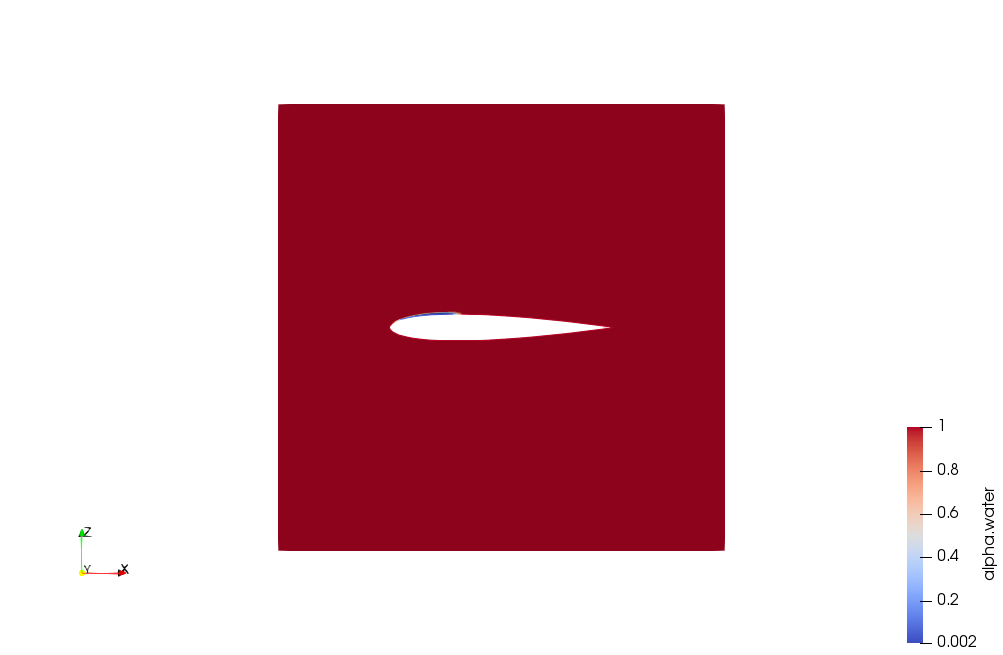
\includegraphics[width=0.3\textwidth]{AOA3.2p/AOA3.2t1alpha}}
    \qquad
  \subfloat[$3.5^{\circ}$]{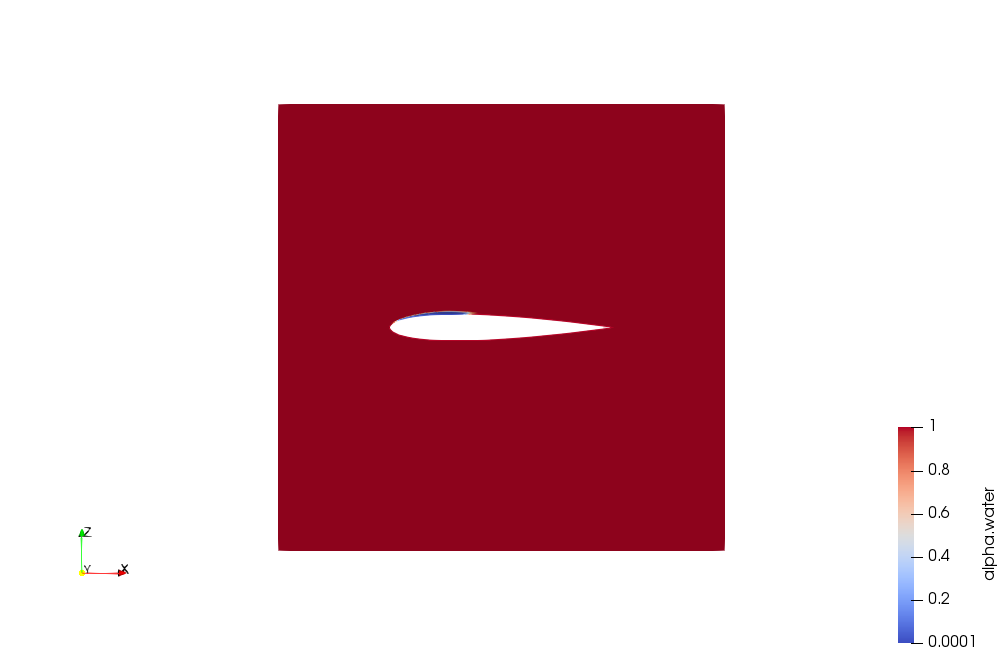
\includegraphics[width=0.3\textwidth]{AOA3.5p/AOA3.5t1alpha}}
   \qquad
  \subfloat[$3.8^{\circ}$]{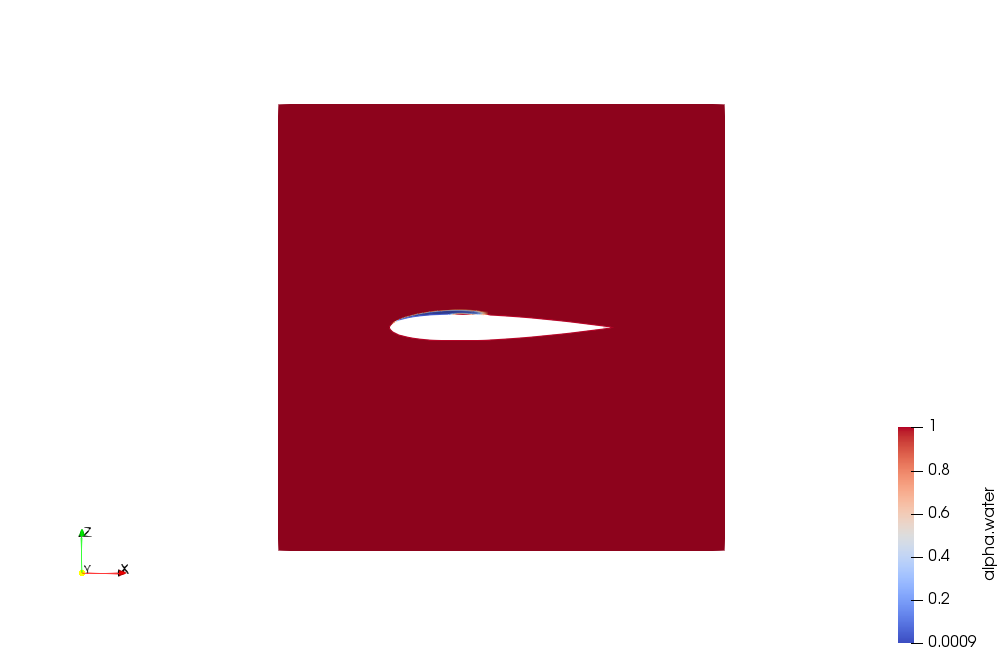
\includegraphics[width=0.3\textwidth]{AOA3.8p/AOA3.8t1alpha}}
      \caption{alpha.water variation over a NACA0012, non cavitating flow}
    \label{fig:fig16}
\end{figure}
 \begin{figure}[H]
    \centering
    \subfloat[$3.2^{\circ}$]{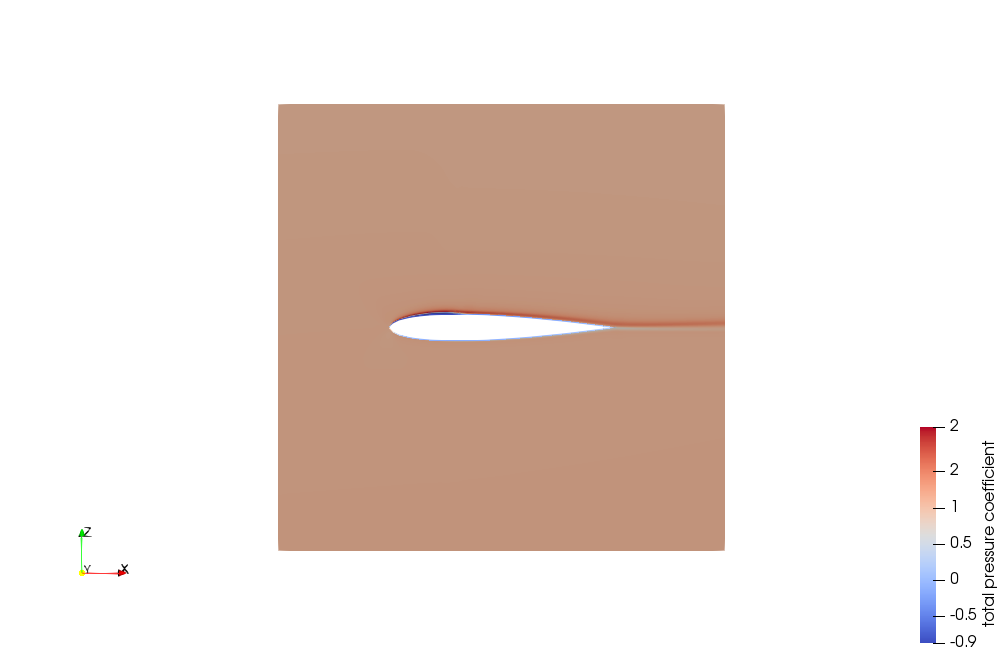
\includegraphics[width=0.3\textwidth]{AOA3.2p/AOA3.2t1cp}}
    \qquad
  \subfloat[$3.5^{\circ}$]{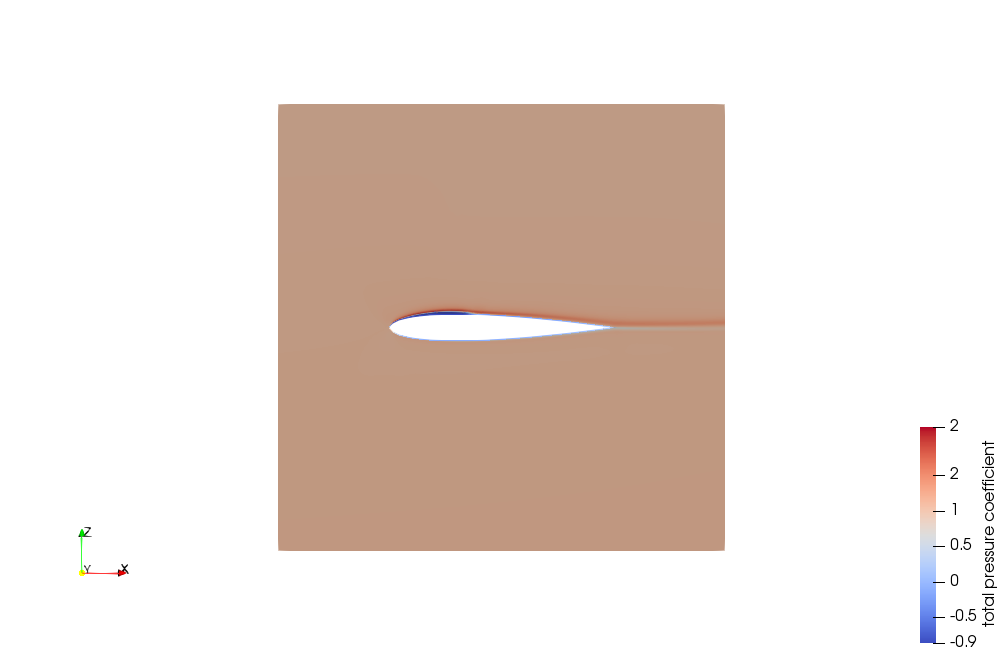
\includegraphics[width=0.3\textwidth]{AOA3.5p/AOA3.5t1cp}}
   \qquad
  \subfloat[$3.8^{\circ}$]{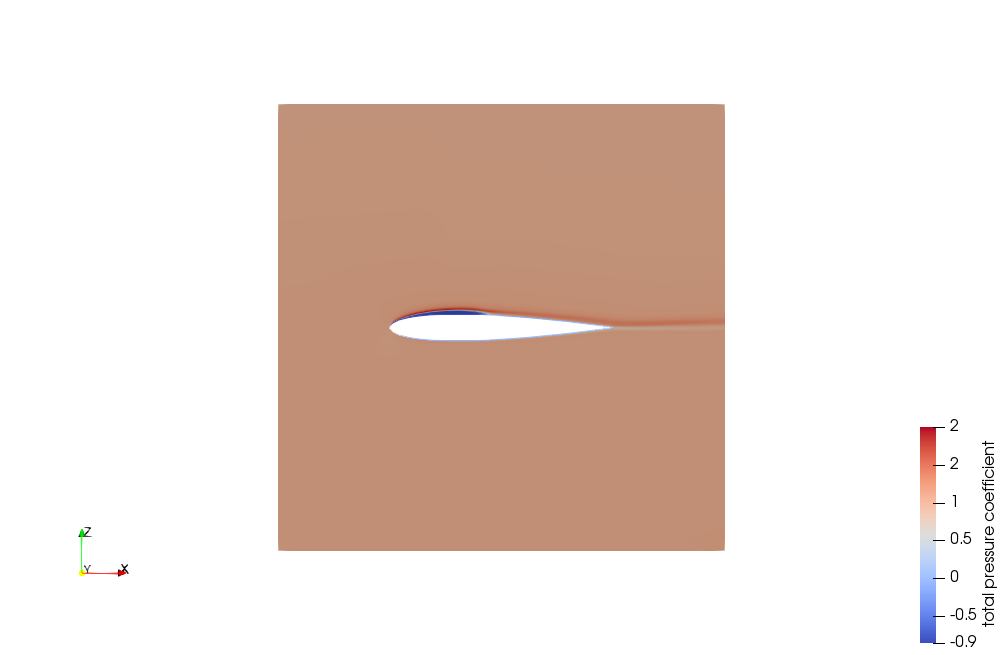
\includegraphics[width=0.3\textwidth]{AOA3.8p/AOA3.8t1cp}}
      \caption{Change in pressure coefficient over a NACA0012, non cavitating flow}
    \label{fig:fig16}
\end{figure} 
  
 \begin{figure}[H]
    \centering
    \subfloat[$3.2^{\circ}$]{\includegraphics[width=0.3\textwidth]{thesisgraph/AOA3.2cp}}
    \qquad
  \subfloat[$3.5^{\circ}$]{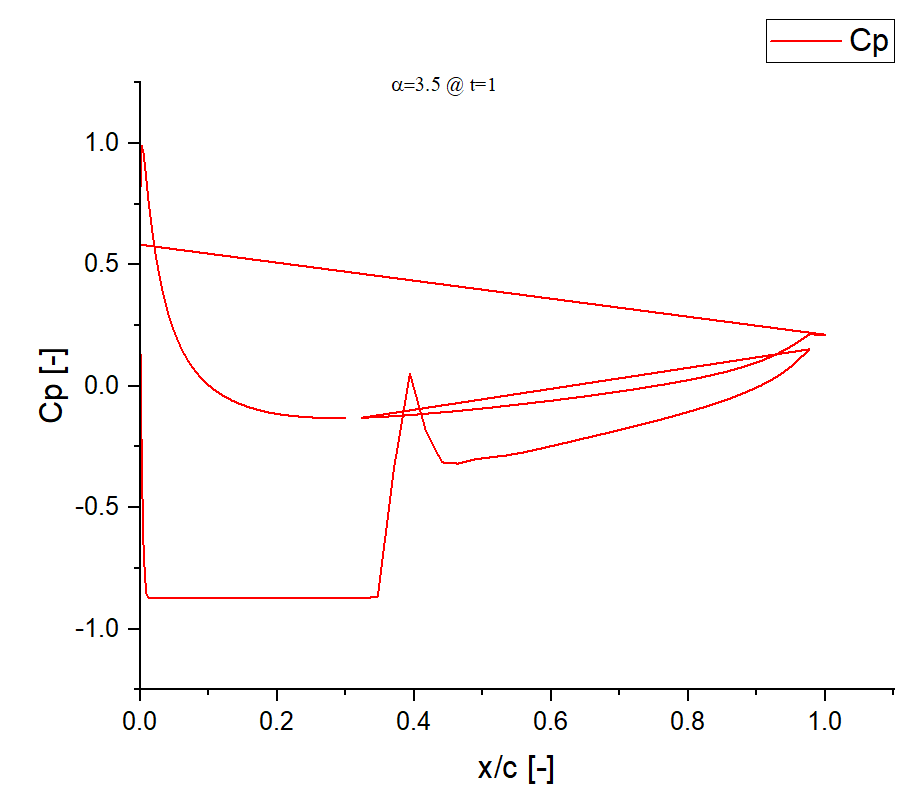
\includegraphics[width=0.3\textwidth]{thesisgraph/AOA3.5cp}}
   \qquad
  \subfloat[$3.8^{\circ}$]{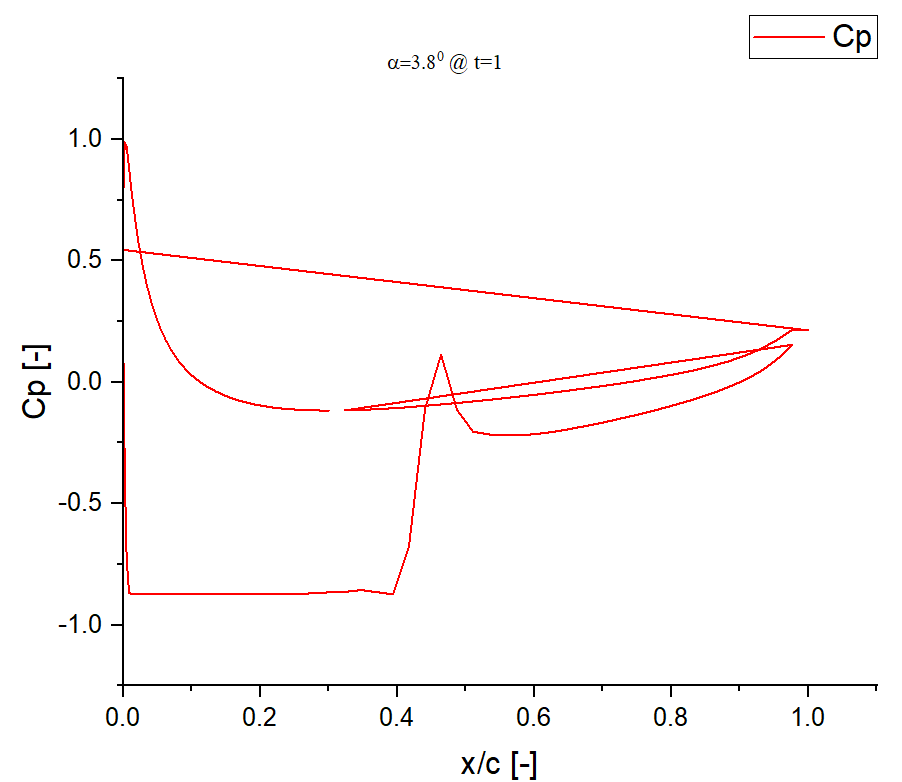
\includegraphics[width=0.3\textwidth]{thesisgraph/AOA3.8cp}}
      \caption{$C_p$ vs x/c for a NACA0012 for non-cavitation flow}
    \label{fig:fig16}
\end{figure} 
   
  \begin{figure}[H]
    \centering
    \subfloat[$3.2^{\circ}$]{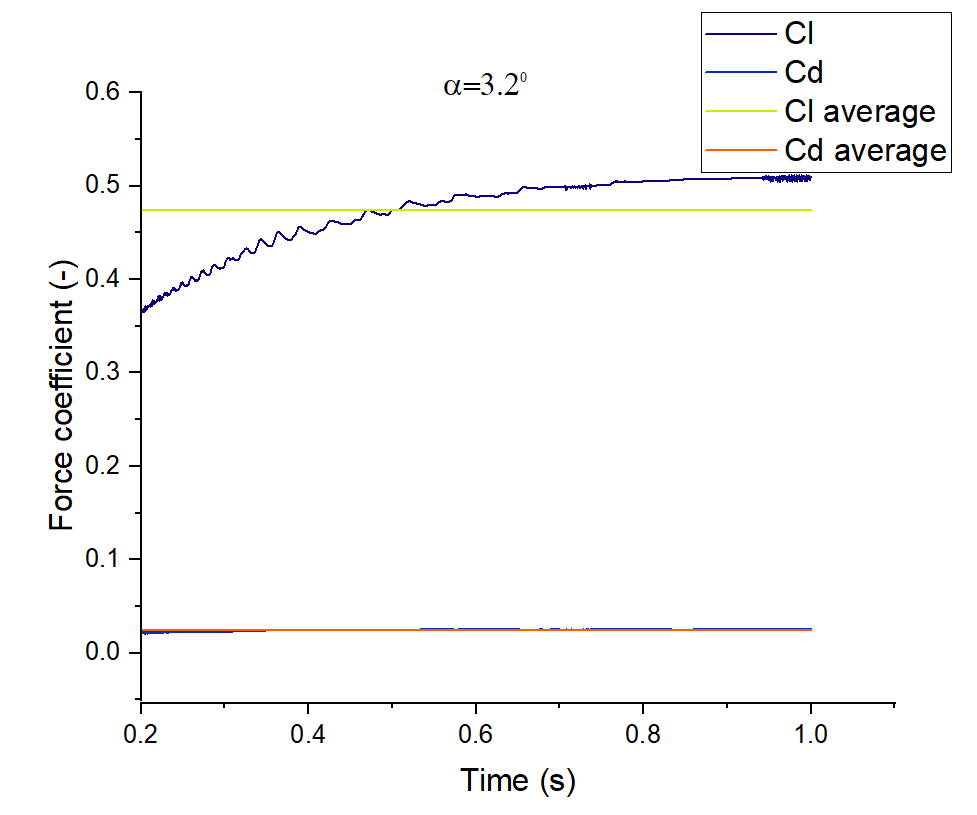
\includegraphics[width=0.3\textwidth]{thesisgraph/AOA3.2forcecoefficient}}
    \qquad
  \subfloat[$3.5^{\circ}$]{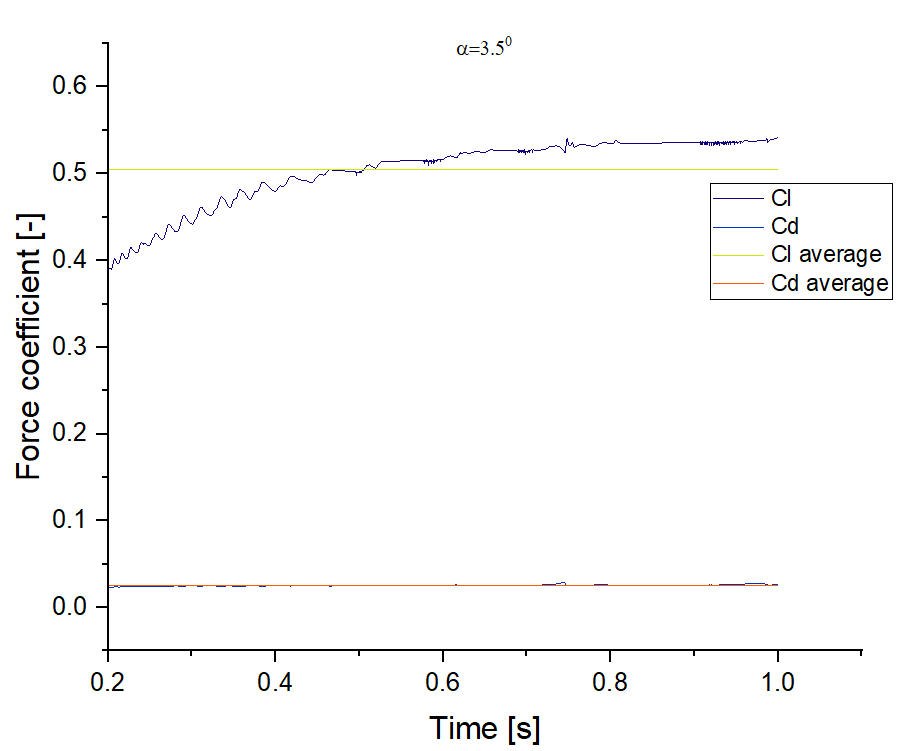
\includegraphics[width=0.3\textwidth]{thesisgraph/AOA3.5forcecoefficient}}
   \qquad
  \subfloat[$3.8^{\circ}$]{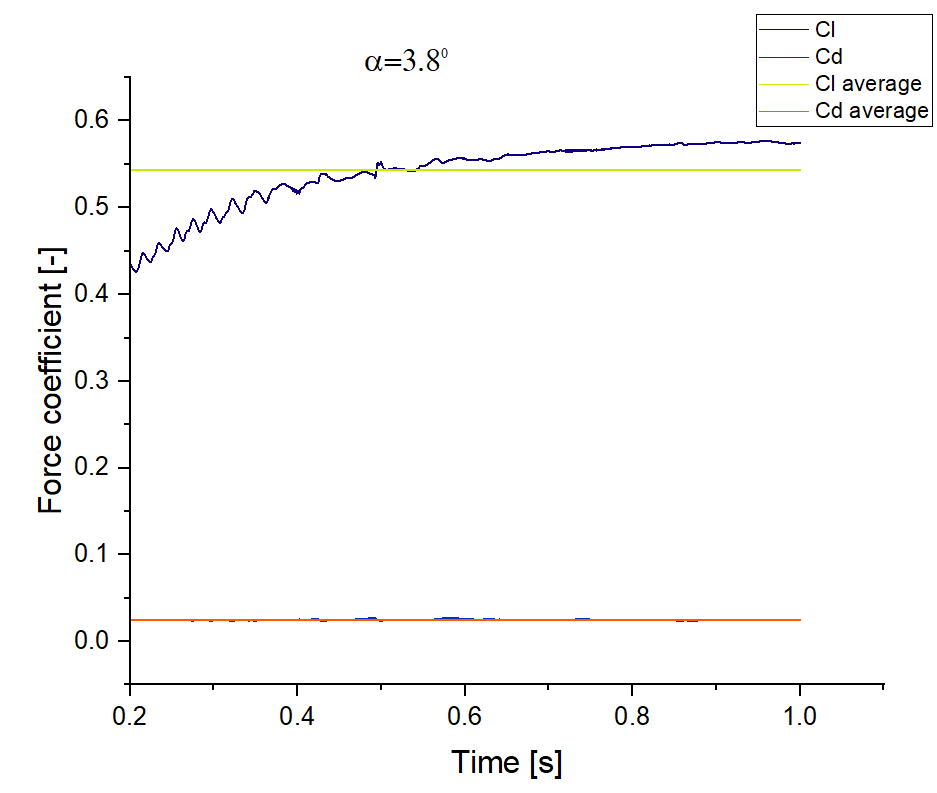
\includegraphics[width=0.3\textwidth]{thesisgraph/AOA3.8forcecoefficient}}
      \caption{Variation of lift and drag coefficient with time on NACA0012, non cavitating flow}
    \label{fig:fig16}
\end{figure} 
\section{Cavitation unsteady flow}
\textbf{Re-entrant jet without shedding}:
 \textbf{AOA 4.1 to AOA 5.0}: A description of cavitation physics and the conditions for closed-type partial
cavitation appears in chapter 1, along with discussions of re-entrant jet phenomena. As long as we keep 
all such conditions in mind, we can observe that, initially, tiny voids and droplets of small thickness 
were produced at the head of the hydrofoil. During that time, the cavity was still attached to the surface 
of the hydrofoil. As time progresses, the attached cavity moves towards the hydrofoil's tail. The cavity's 
thickness gradually increased along the wing chord until it reached its maximum and experienced a re-entrant 
jet in table (4.3). Hence, this re-entrant jet is due to the minimum pressure occurring inside the cavity itself, 
so the curvature of the streamlines around it tends to direct towards the cavity. The re-entrant jet is so energized then only it can cut the cavity interface.
However, there was no shedding of an unsteady vapor cloud as shown in table (4.4). The cavity was divided into two parts. 
The first part was often attached to the leading edge of  suction side of the hydrofoil and the region ${(1/4)}^{th}$ of the chord will be highly 
influenced by the re-entrant jet. After a while when the re-entrant jet crosses the rear area and moves towards the leading edge 
the rear area gets suddenly reattached to the surface due to turbulent reattachment.\\
\textbf{Re-entrant jet with unsteady cloud shedding}:  
\textbf{AOA 5.7 to AOA 8}: A sheet cavity with purely filled vapor appeared at the front of the suction side of the hydrofoil. 
The thickness of the cavity increases gradually and starts moving downward. The end of the cavity 
was located at the tail of the hydrofoil. The front part close to the leading edge is attached to the surface and the 
tail part of the cavity fell off and moved downstream. As we can see from the table (4.4), there is periodic shedding take 
place after a regular interval of time once the cavity length and thickness of the cavity decrease. 
Because of the unbalanced flow field and development of the low-pressure zone, the sheet cavity was further expanded.
 This means once the thickness of the cavity reduces after a shedding the 
cavity grows again and reaches its maximum, then the re-entrant jet from the table (4.3) cut the cavity interface and 
moved towards the leading edge, and then cloud shedding takes place. As we closely observed the alpha.water table (4.4) it can be seen that once the cavity 
break near the $(1/3)^{th}$ of the chord there is turbulent reattachment taking place near the tail of the suction side of the hydrofoil.
As time progresses the wake completely filled with vapor and separated vortices at the tail of the hydrofoil were very obvious. 

 
  
  
\begin{table}[h]
\centering
 \begin{figure}[H]
\begin{tabular}{|llll|}
\hline
\rowcolor{gray!20} \multicolumn{4}{|l|}{Velocity distribution for a different angles of attack}\\ \hline
\multicolumn{1}{|l|}{$\alpha={{4.1}^{\circ}}$} & \multicolumn{1}{l|}{\subfloat[t=0.6 s]{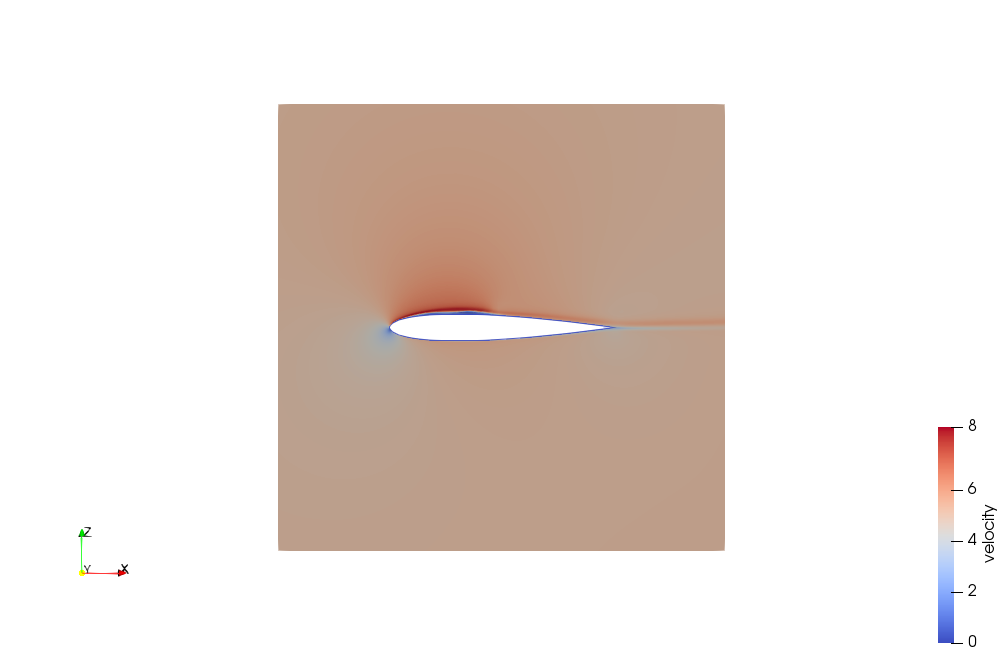
\includegraphics[width=0.3\textwidth]{AOA4.1p/AOA4.1t0.6v}}} 
& \multicolumn{1}{l|}{\subfloat[t=0.8 s]{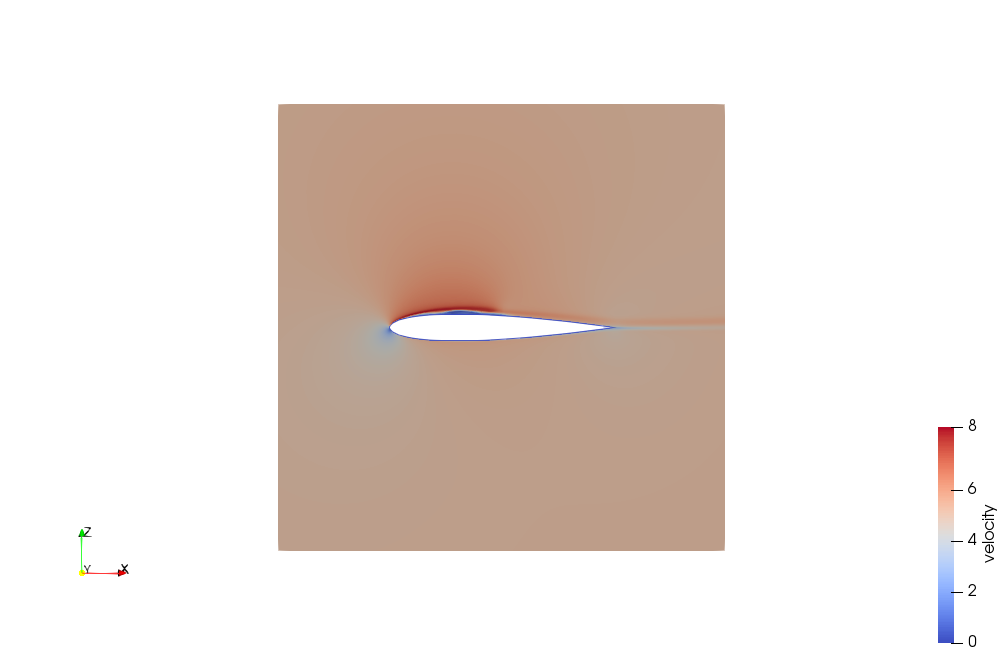
\includegraphics[width=0.3\textwidth]{AOA4.1p/AOA4.1t0.8v}}} &\subfloat[t=1 s]{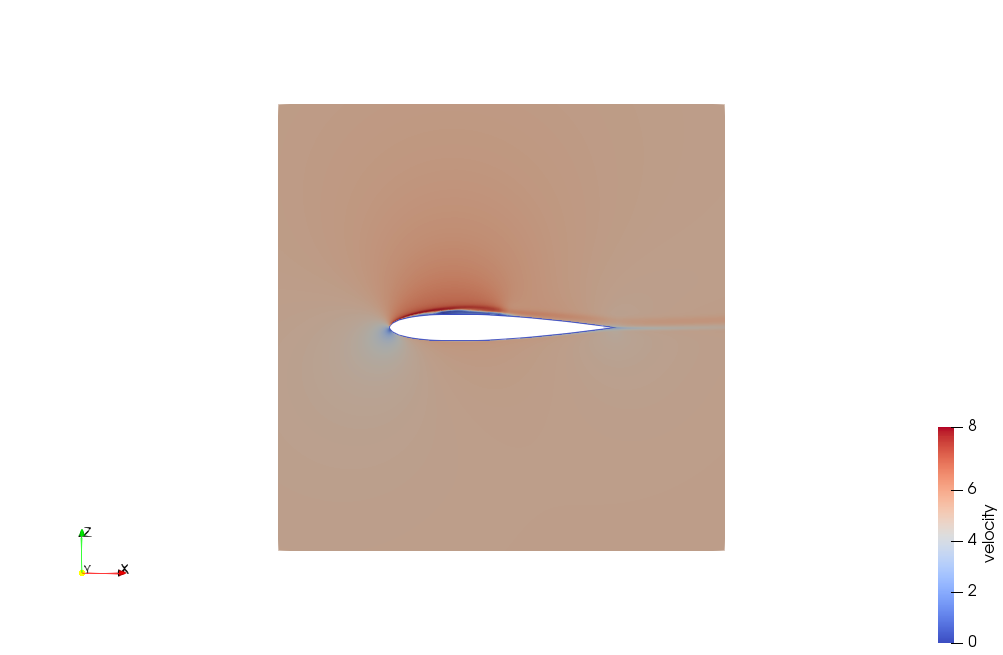
\includegraphics[width=0.3\textwidth]{AOA4.1p/AOA4.1t1v}}  \\ \hline

\multicolumn{1}{|l|}{$\alpha={{4.5}^{\circ}}$} & \multicolumn{1}{l|}{\subfloat[t=0.42 s]{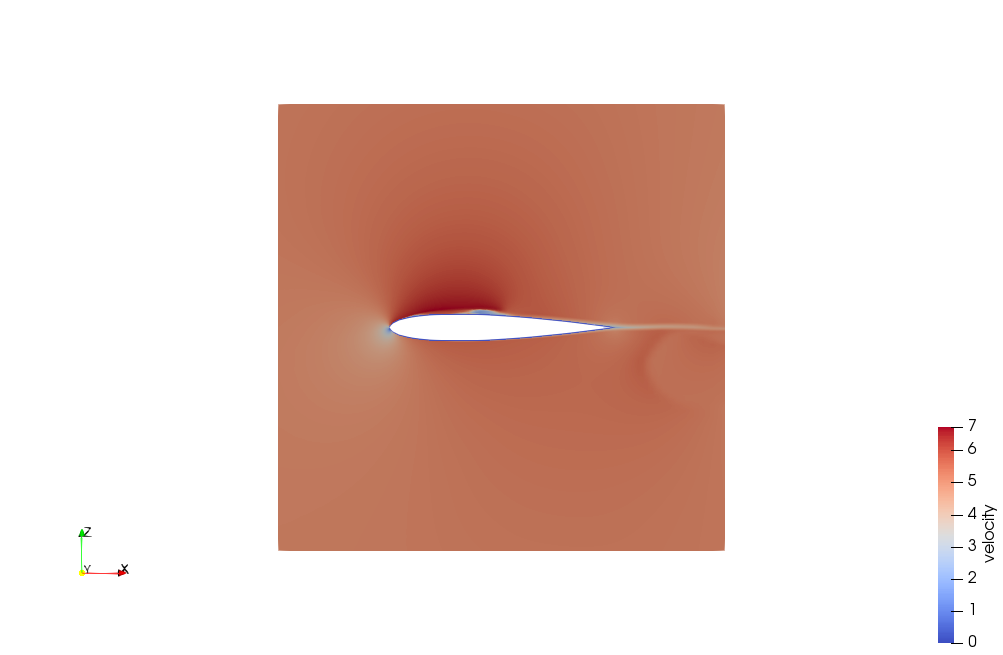
\includegraphics[width=0.3\textwidth]{AOA4.5p/AOA4.5t0.42v}}} 
& \multicolumn{1}{l|}{\subfloat[t=0.66 s]{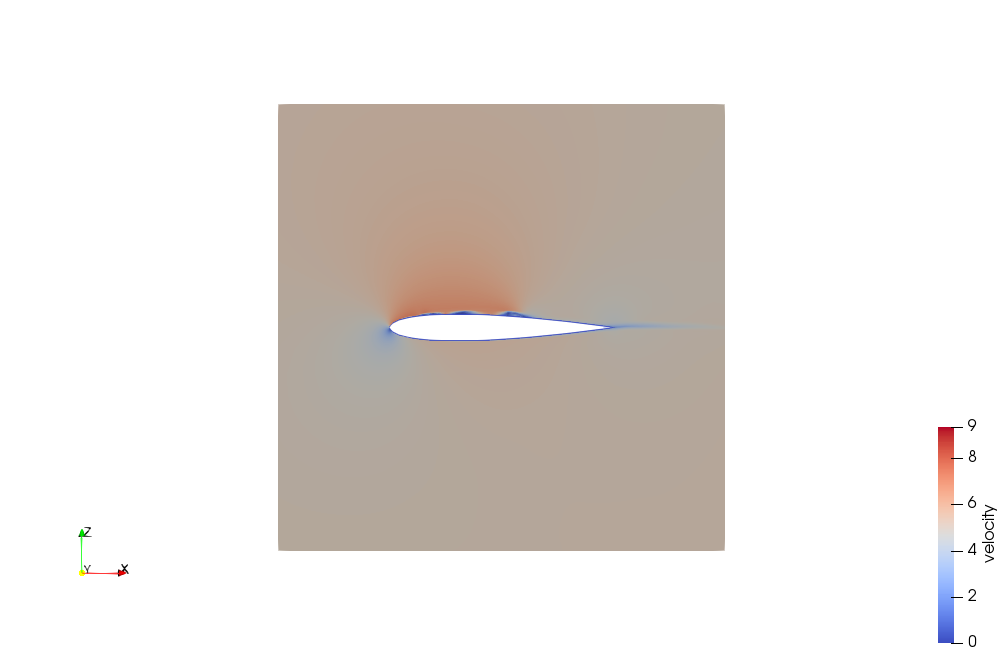
\includegraphics[width=0.3\textwidth]{AOA4.5p/AOA4.5t0.66v}}} & {\subfloat[t=0.72 s]{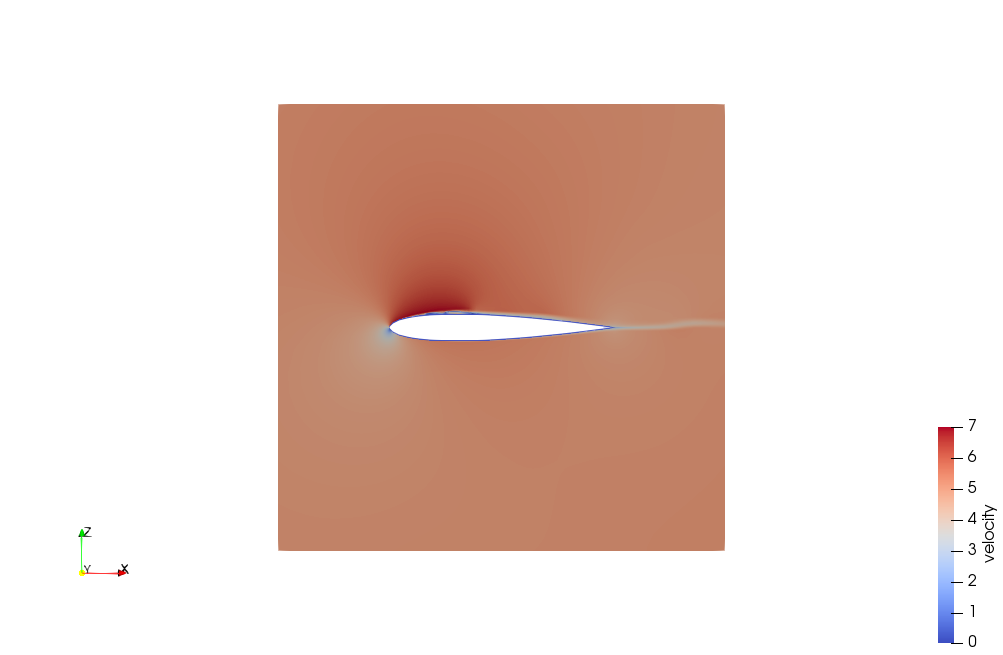
\includegraphics[width=0.3\textwidth]{AOA4.5p/AOA4.5t0.72v}}} \\ \hline

\multicolumn{1}{|l|}{$\alpha={{5.0}^{\circ}}$} & \multicolumn{1}{l|}{\subfloat[t=0.5 s]{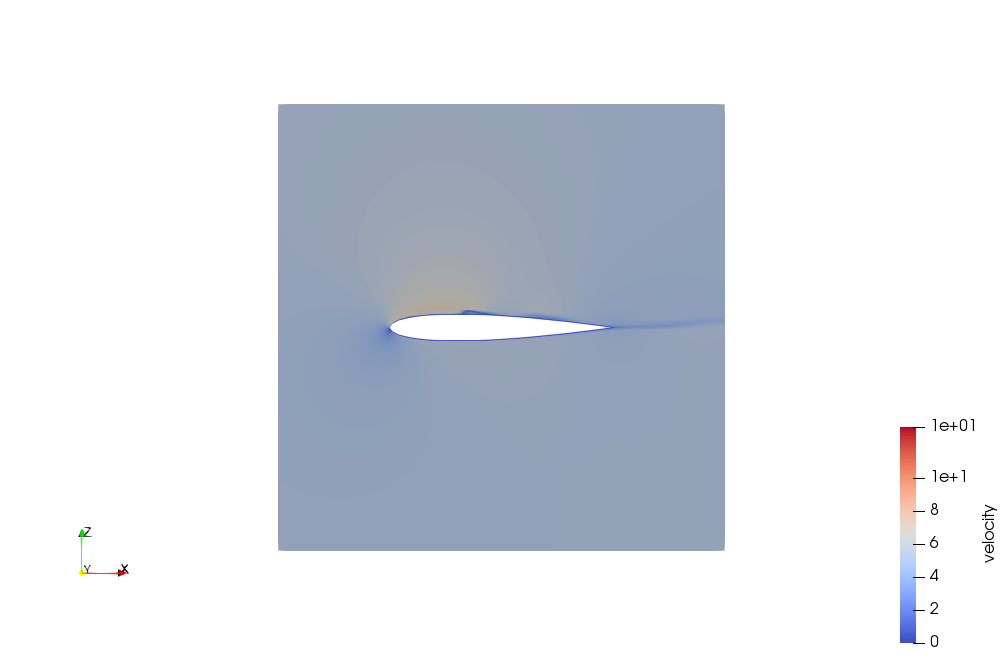
\includegraphics[width=0.3\textwidth]{AOA5p/AOA5.0t0.5v}}} 
& \multicolumn{1}{l|}{\subfloat[t=0.7 s]{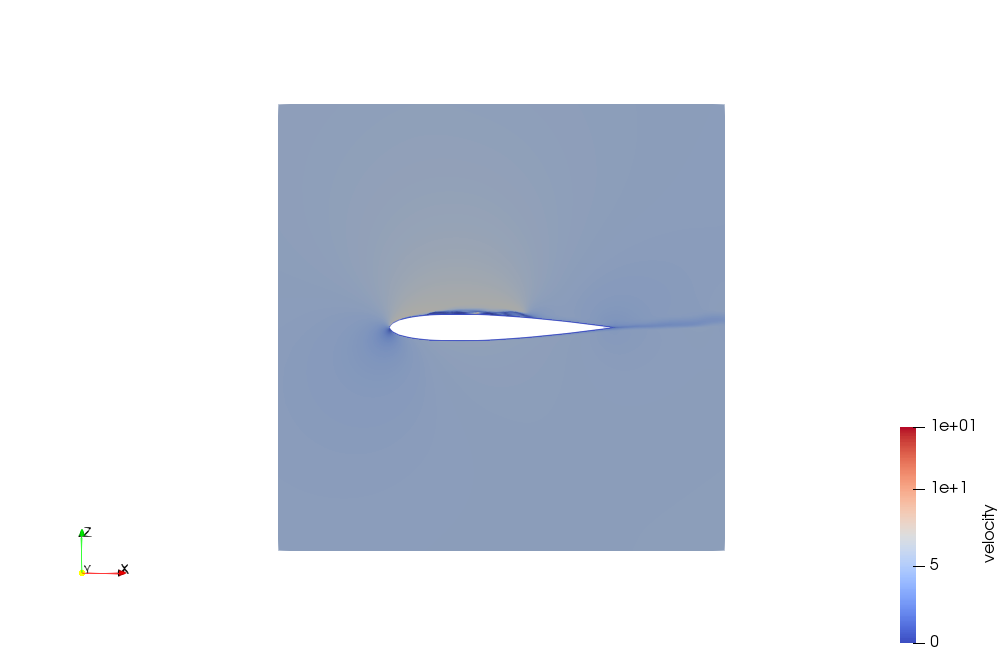
\includegraphics[width=0.3\textwidth]{AOA5p/AOA5.0t0.7v}}} &\subfloat[t=0.88 s]{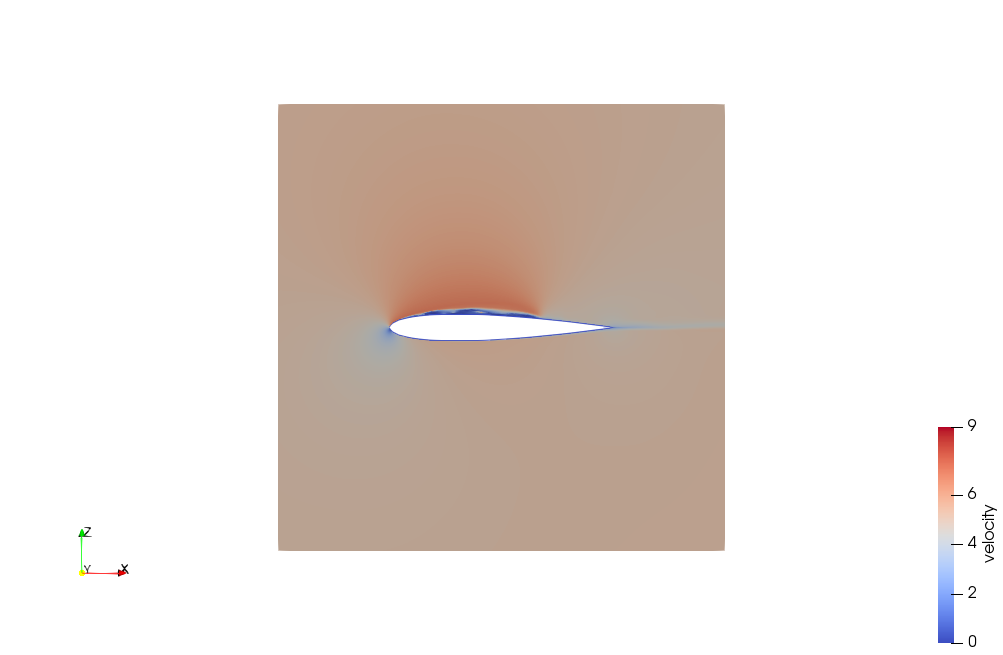
\includegraphics[width=0.3\textwidth]{AOA5p/AOA5.0t0.88v}}  \\ \hline

\multicolumn{1}{|l|}{$\alpha={{5.7}^{\circ}}$} & \multicolumn{1}{l|}{\subfloat[t=0.7 s]{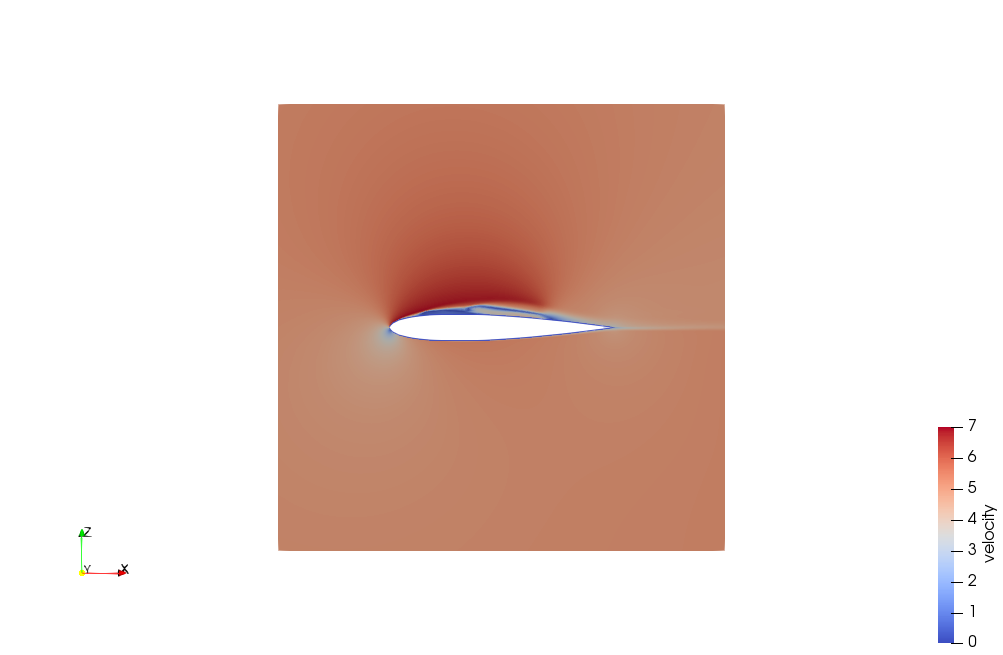
\includegraphics[width=0.3\textwidth]{AOA5.7p/AOA5.7t0.7v}}} 
& \multicolumn{1}{l|}{\subfloat[t=0.8 s]{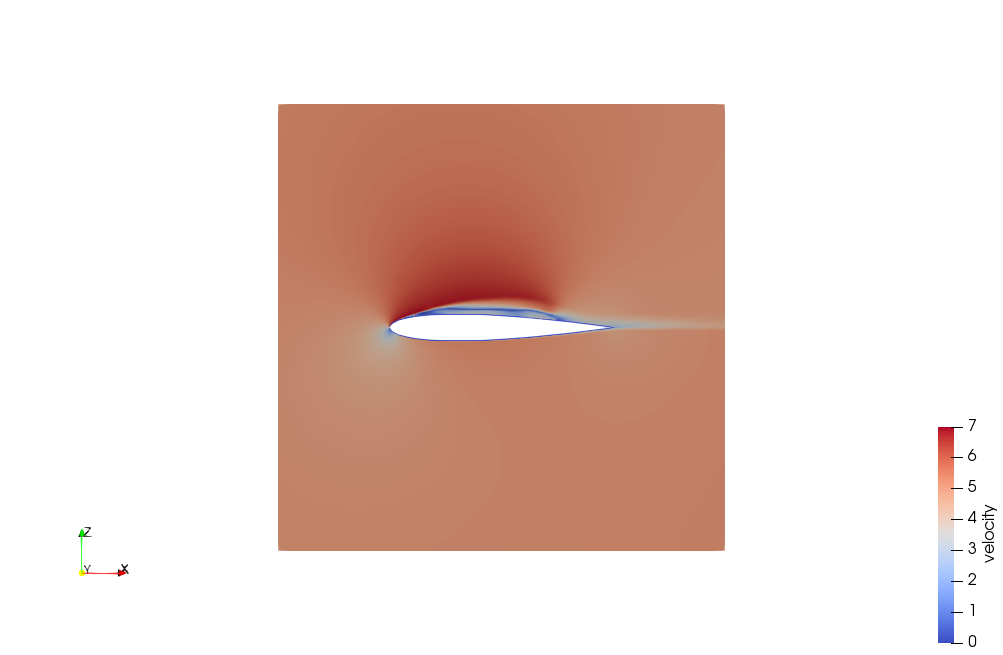
\includegraphics[width=0.3\textwidth]{AOA5.7p/AOA5.7t0.8v}}} &\subfloat[t=1 s]{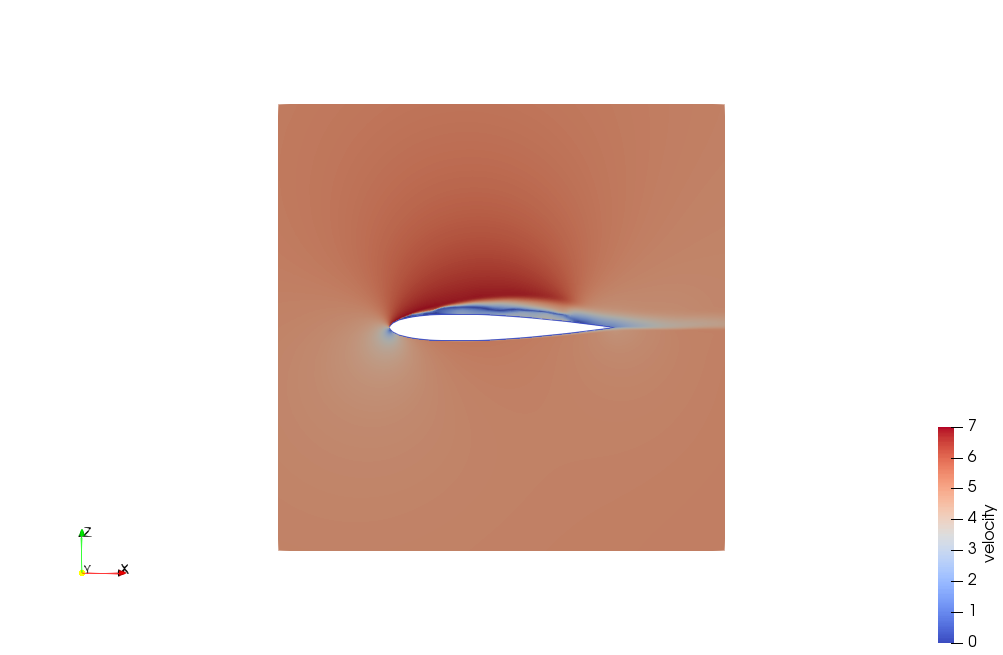
\includegraphics[width=0.3\textwidth]{AOA5.7p/AOA5.7t1v}}  \\ \hline

\multicolumn{1}{|l|}{$\alpha={{6.5}^{\circ}}$} & \multicolumn{1}{l|}{\subfloat[t=0.8 s]{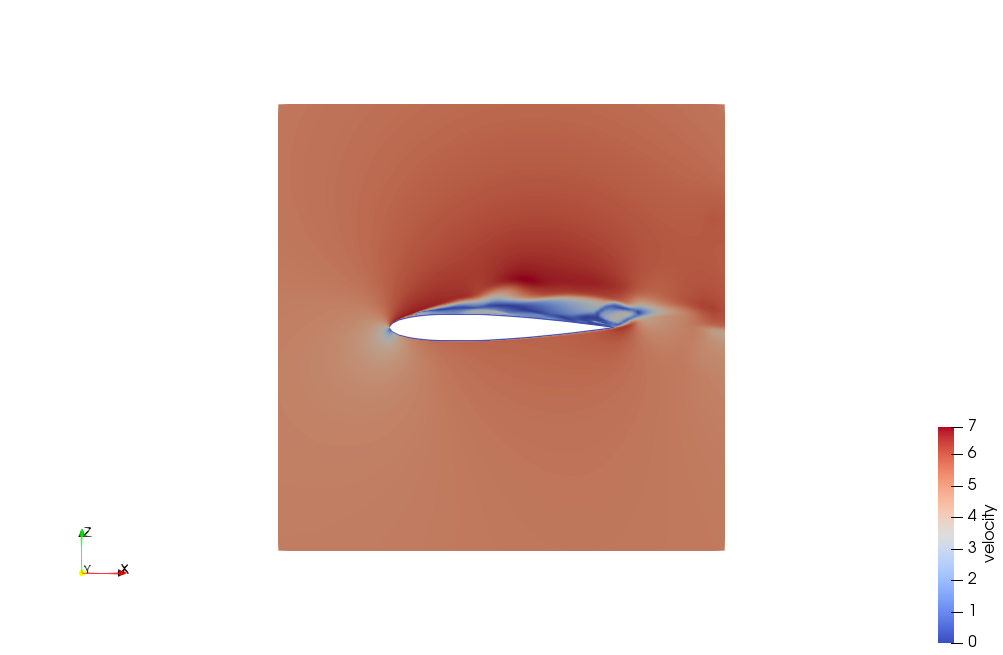
\includegraphics[width=0.3\textwidth]{AOA6.5p/AOA6.5t0.8v}}} 
& \multicolumn{1}{l|}{\subfloat[t=0.9 s]{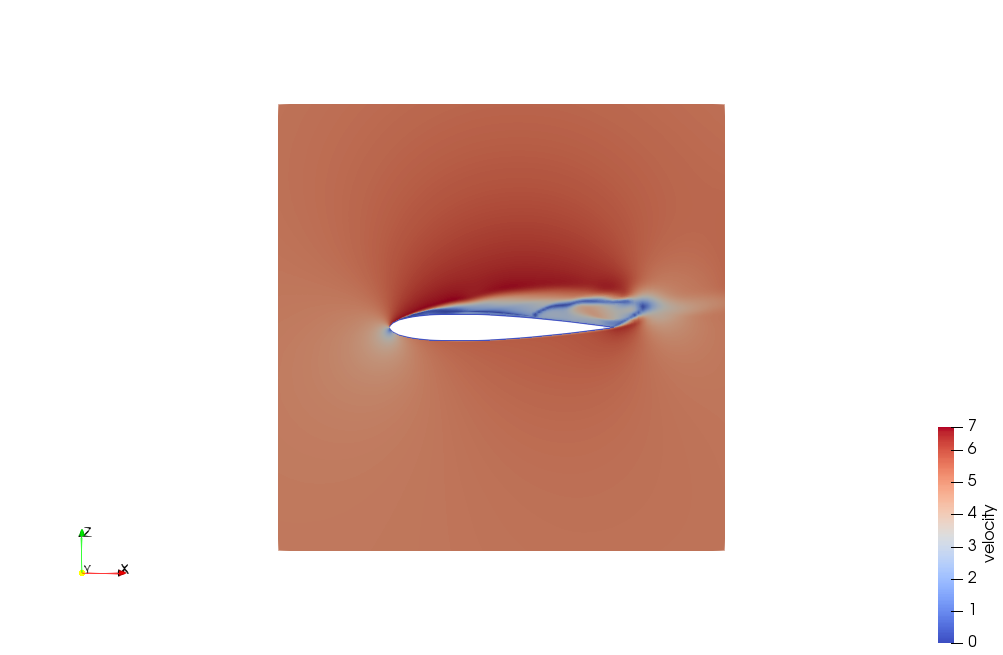
\includegraphics[width=0.3\textwidth]{AOA6.5p/AOA6.5t0.9v}}} &\subfloat[t=1 s]{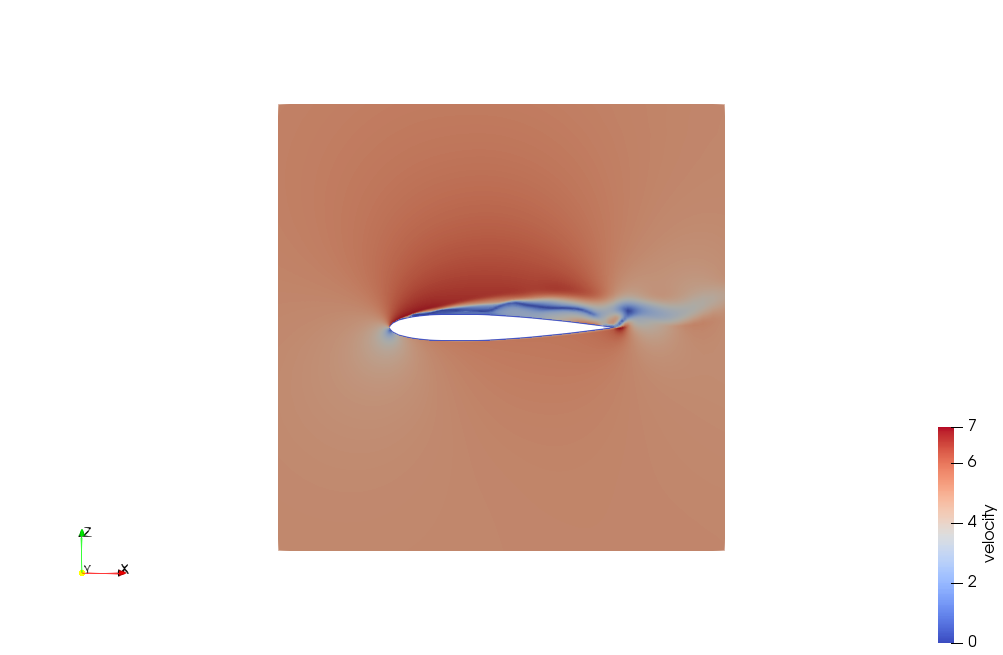
\includegraphics[width=0.3\textwidth]{AOA6.5p/AOA6.5t1v}}  \\ \hline

\end{tabular}
\end{figure}
\end{table}
 
 \begin{table}[h]
\centering
 \begin{figure}[H]
\begin{tabular}{|llll|} 
\hline
\rowcolor{gray!20} \multicolumn{4}{|l|}{Velocity distribution for a different angles of attack}\\ \hline
 \multicolumn{1}{|l|}{$\alpha={{7.6}^{\circ}}$} & \multicolumn{1}{l|}{\subfloat[t=0.6 s]{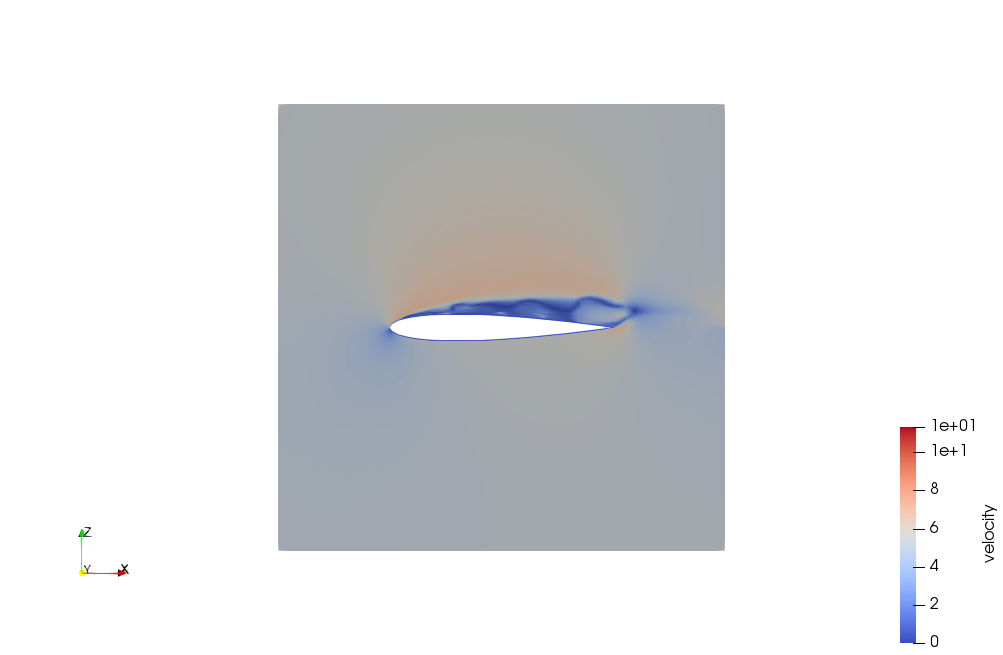
\includegraphics[width=0.3\textwidth]{AOA7.6p/AOA7.6t0.6v}}} 
& \multicolumn{1}{l|}{\subfloat[t=0.82 s]{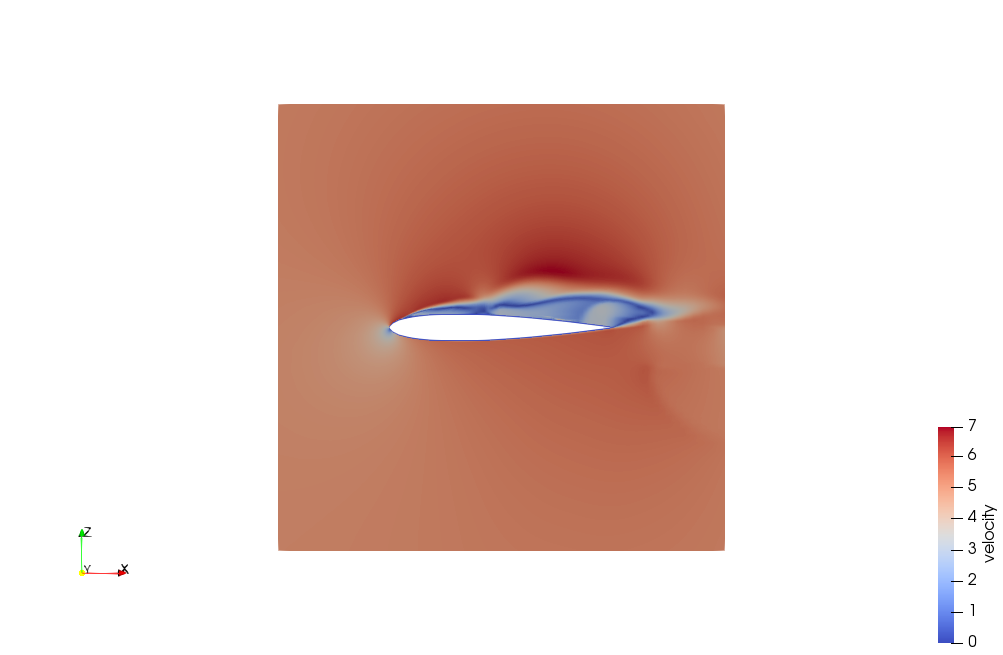
\includegraphics[width=0.3\textwidth]{AOA7.6p/AOA7.6t0.82v}}} &\subfloat[t=0.92 s]{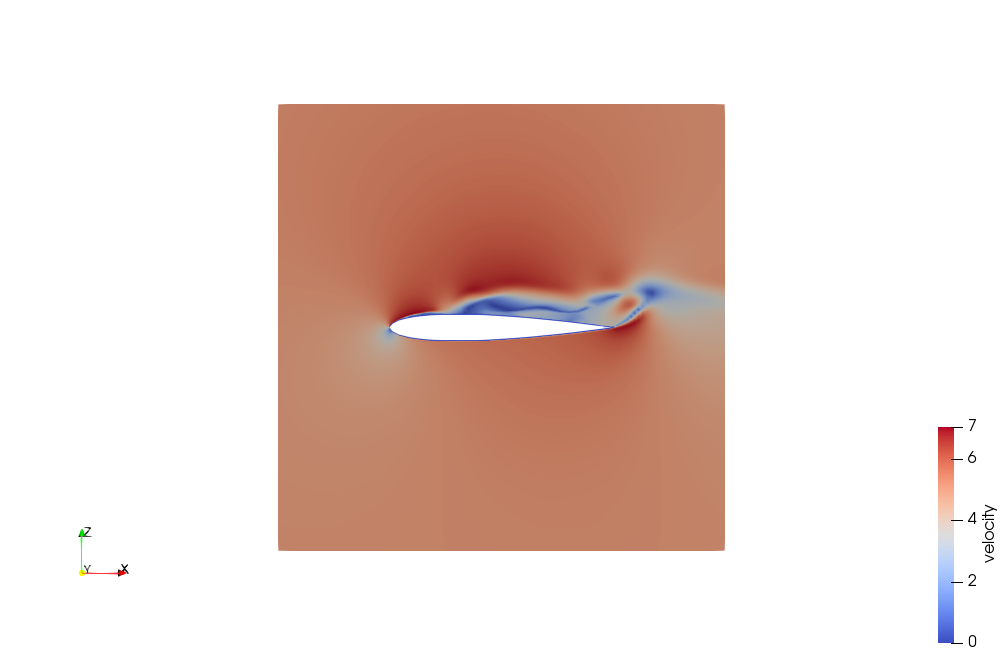
\includegraphics[width=0.3\textwidth]{AOA7.6p/AOA7.6t0.92v}}  \\ \hline


  \multicolumn{1}{|l|}{$\alpha={{8}^{\circ}}$} & \multicolumn{1}{l|}{\subfloat[t=0.5 s]{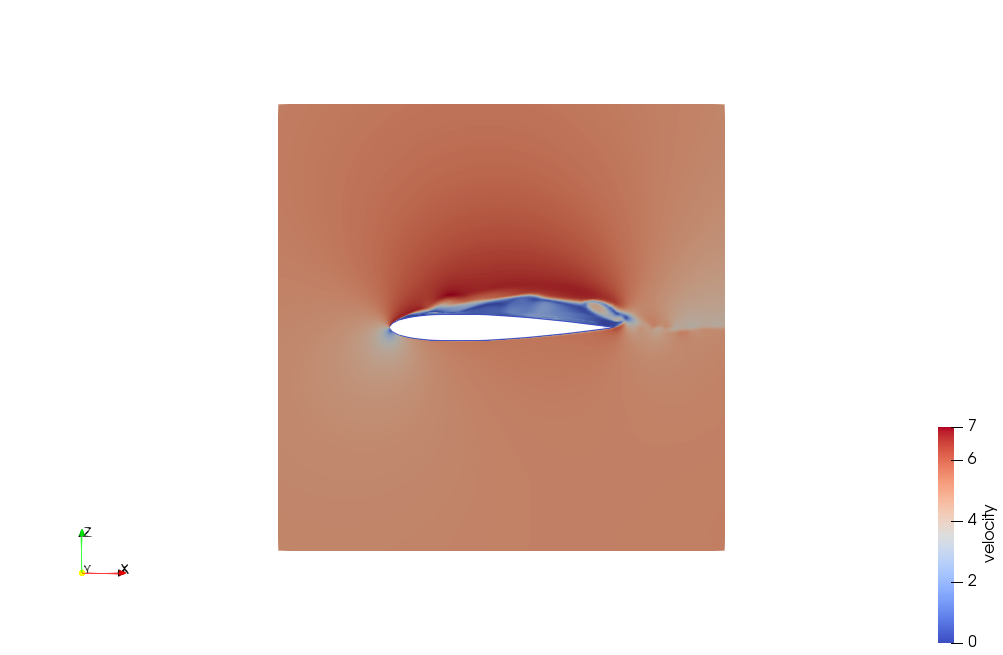
\includegraphics[width=0.3\textwidth]{AOA8p/AOA8t0.5v}}} 
& \multicolumn{1}{l|}{\subfloat[t=0.7 s]{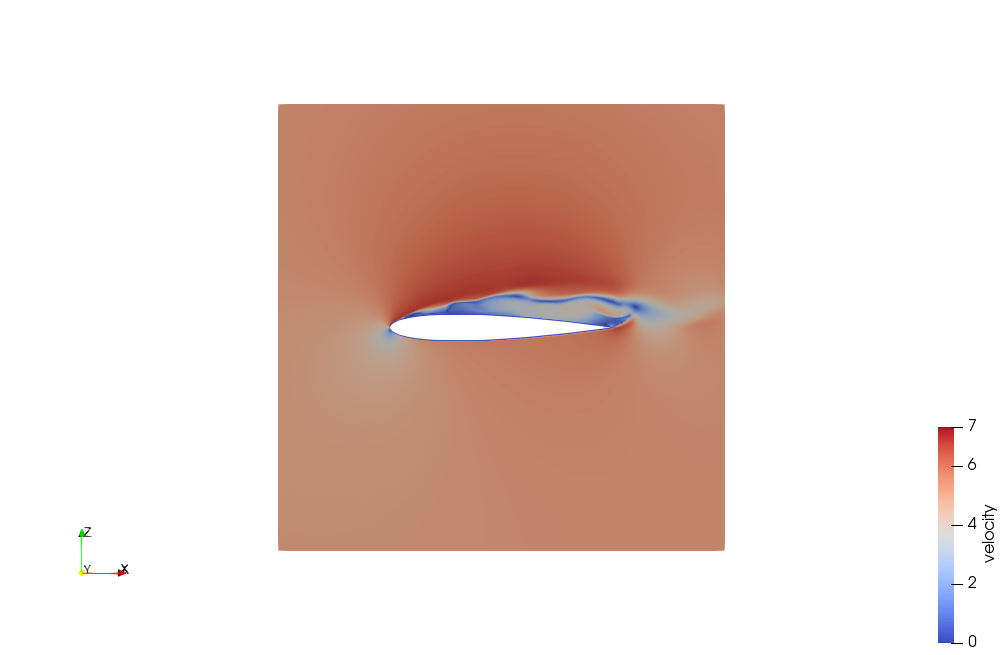
\includegraphics[width=0.3\textwidth]{AOA8p/AOA8t0.7v}}} &\subfloat[t=0.9 s]{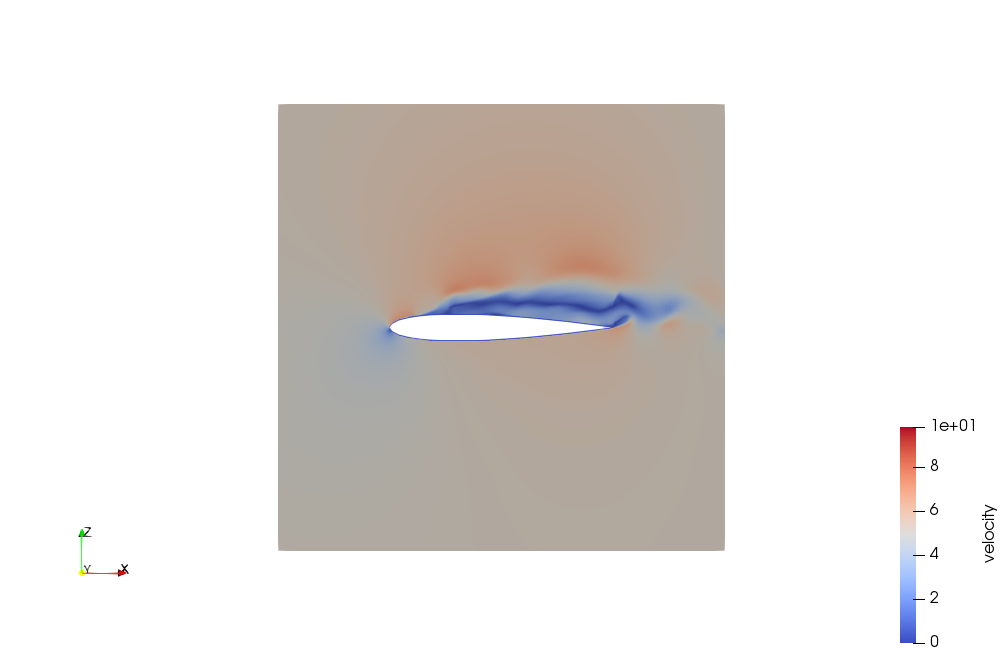
\includegraphics[width=0.3\textwidth]{AOA8p/AOA8t0.9v}}  \\ \hline
\end{tabular}
\end{figure}
\caption{Velocity distribution over a NACA0012 hydrofoil at different angles of attack and time period}
 \label{fig:fig16}
\end{table}


 \begin{table}[h]
\centering
 \begin{figure}[H]
\begin{tabular}{|llll|}
\hline
\rowcolor{gray!20} \multicolumn{4}{|l|}{Re-entrant at different angles of attack}\\ \hline
\multicolumn{1}{|l|}{$\alpha={{4.1}^{\circ}}$} & \multicolumn{1}{l|}{\subfloat[t=0.6 s]{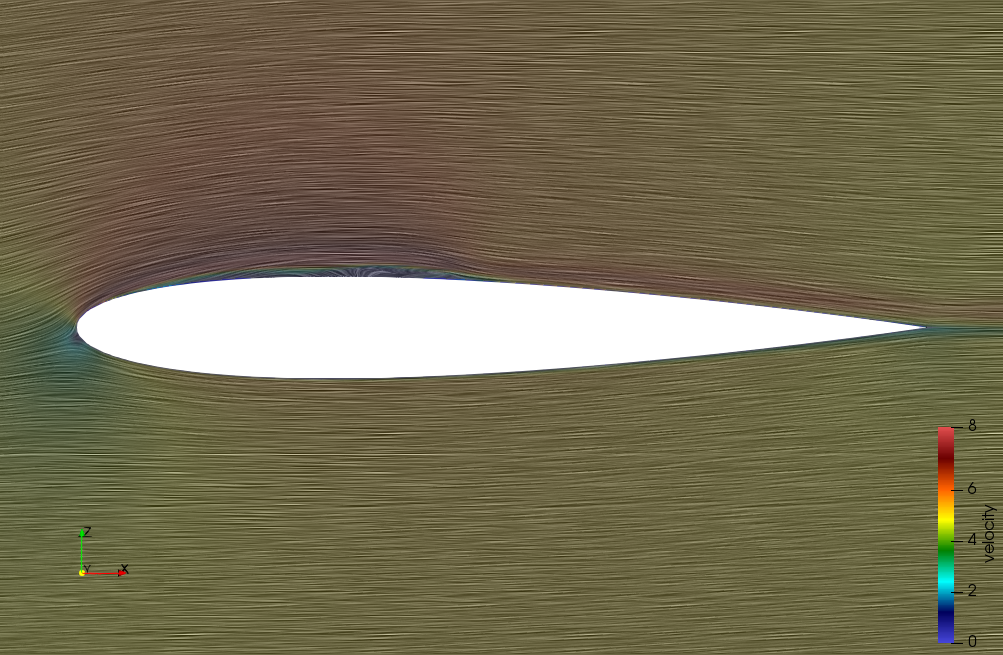
\includegraphics[width=0.3\textwidth]{AOA4.1p/AOA4.1t0.6RE}}} 
& \multicolumn{1}{l|}{\subfloat[t=0.8 s]{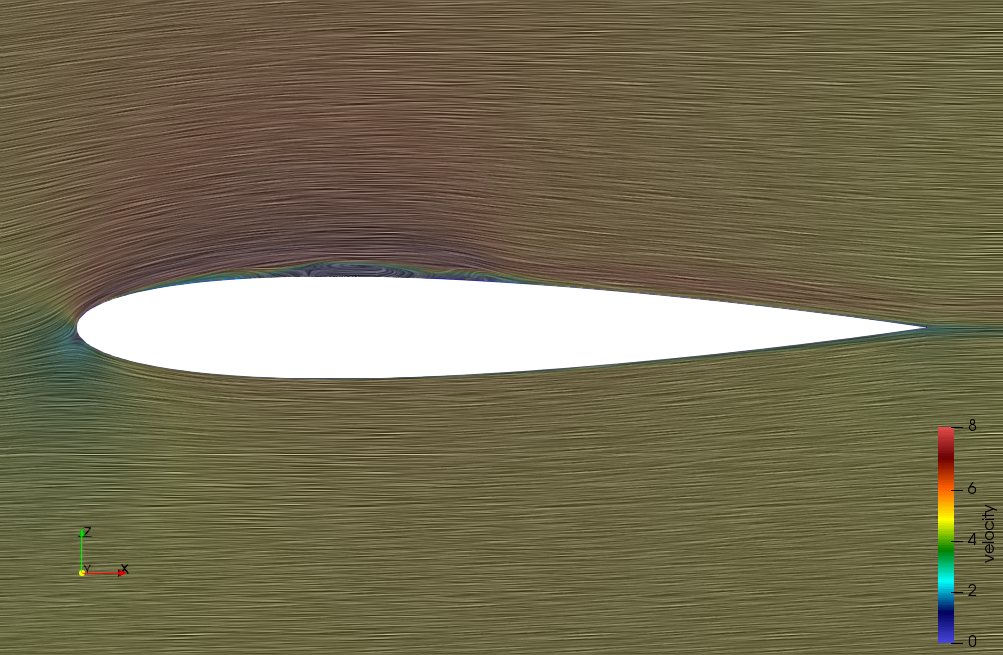
\includegraphics[width=0.3\textwidth]{AOA4.1p/AOA4.1t0.8RE}}} &\subfloat[t=1 s]{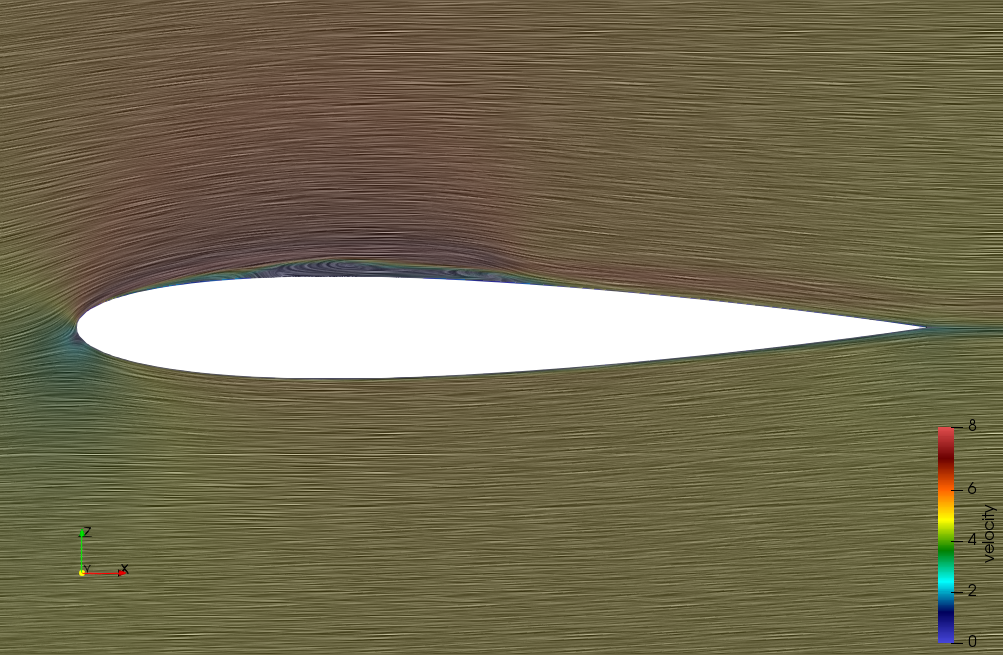
\includegraphics[width=0.3\textwidth]{AOA4.1p/AOA4.1t1RE}}  \\ \hline

\multicolumn{1}{|l|}{$\alpha={{4.5}^{\circ}}$} & \multicolumn{1}{l|}{\subfloat[t=0.42 s]{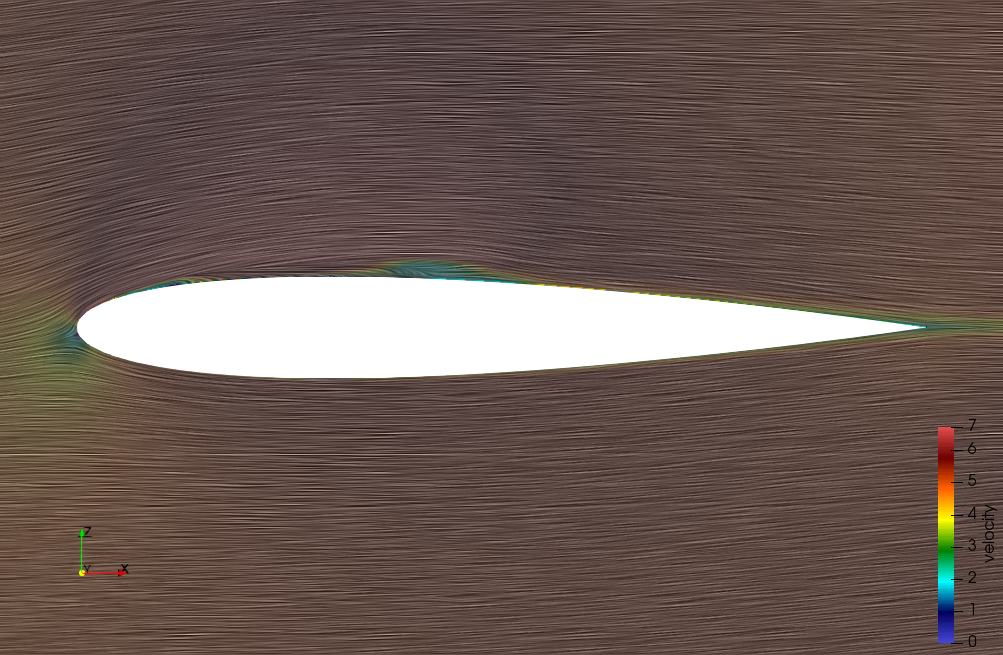
\includegraphics[width=0.3\textwidth]{AOA4.5p/AOA4.5t0.42RE}}} 
& \multicolumn{1}{l|}{\subfloat[t=0.66 s]{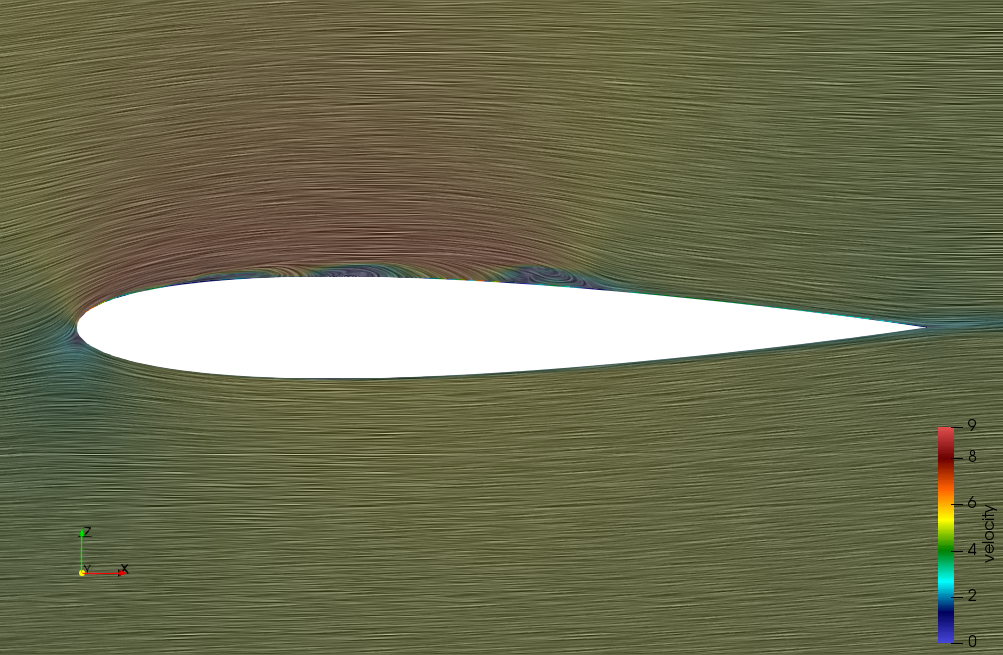
\includegraphics[width=0.3\textwidth]{AOA4.5p/AOA4.5t0.66RE}}} & {\subfloat[t=0.72 s]{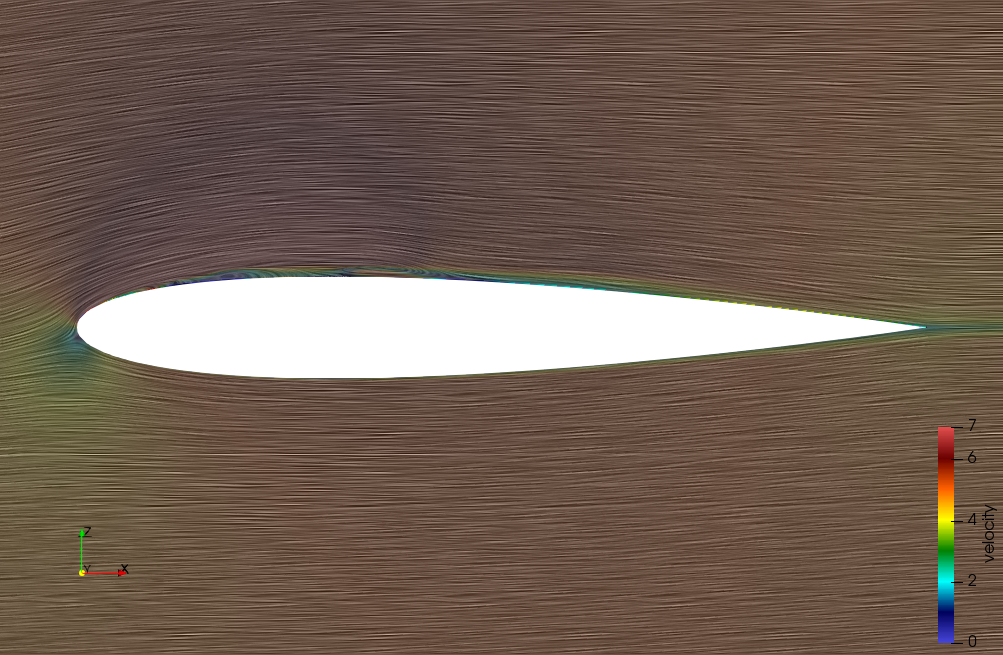
\includegraphics[width=0.3\textwidth]{AOA4.5p/AOA4.5t0.72RE}}} \\ \hline

\multicolumn{1}{|l|}{$\alpha={{5.0}^{\circ}}$} & \multicolumn{1}{l|}{\subfloat[t=0.5 s]{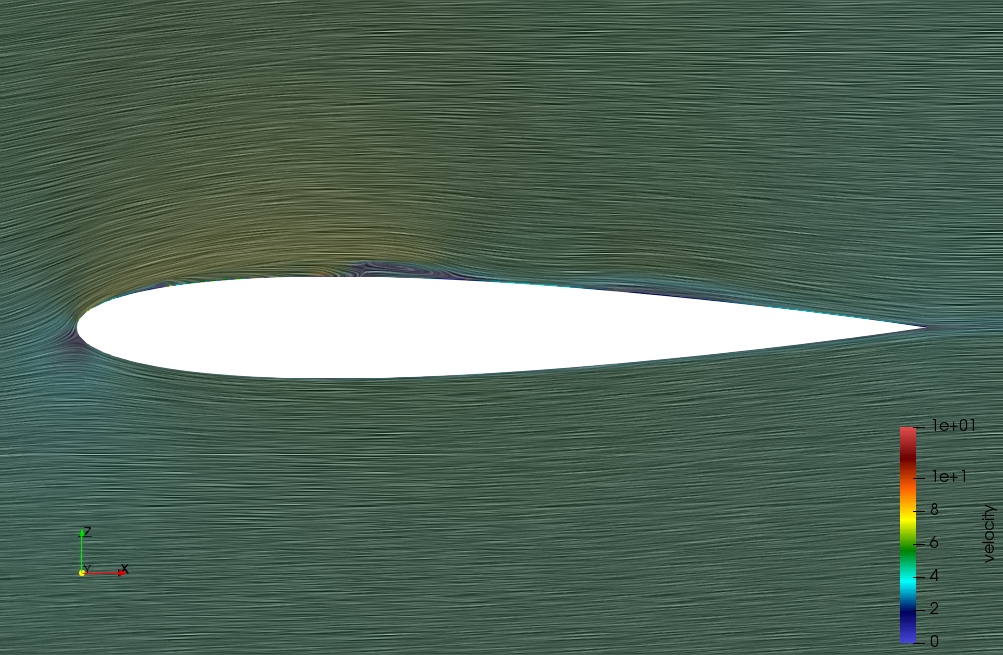
\includegraphics[width=0.3\textwidth]{AOA5p/AOA5.0t0.5RE}}} 
& \multicolumn{1}{l|}{\subfloat[t=0.7 s]{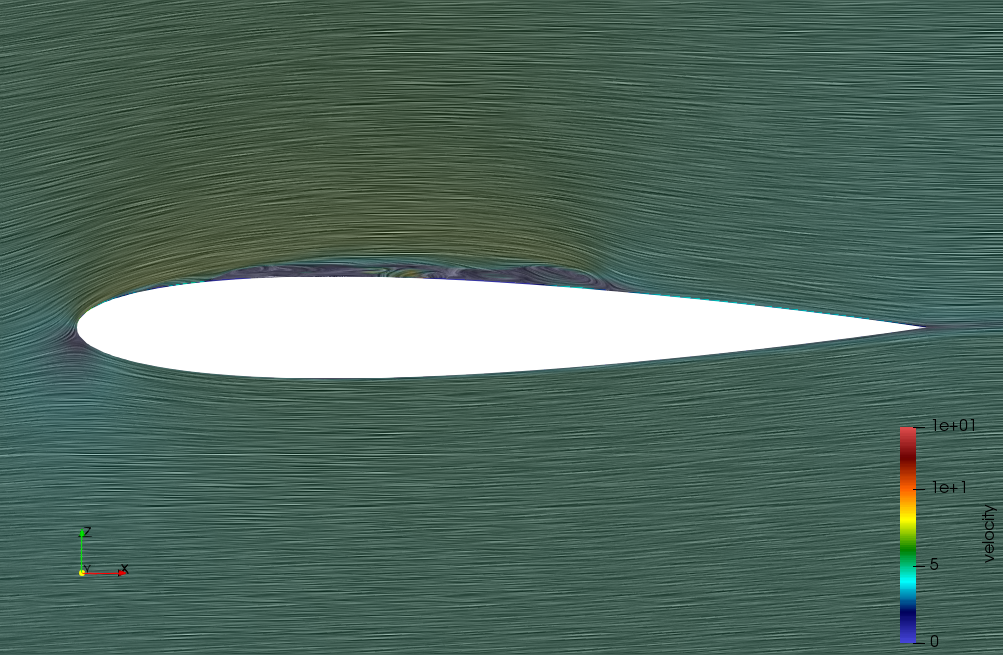
\includegraphics[width=0.3\textwidth]{AOA5p/AOA5.0t0.7RE}}} &\subfloat[t=0.88 s]{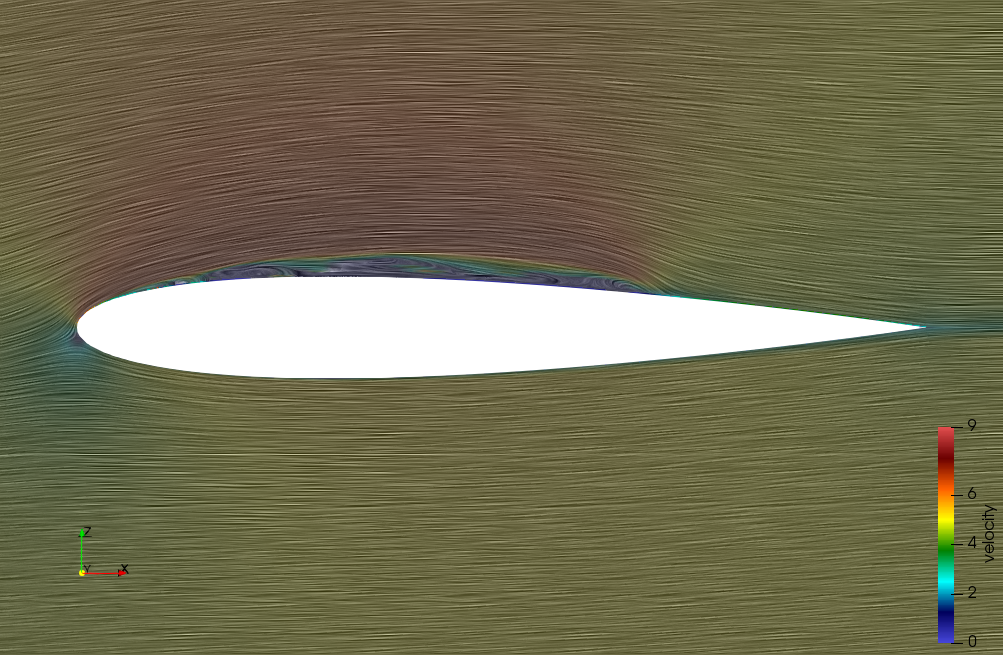
\includegraphics[width=0.3\textwidth]{AOA5p/AOA5.0t0.88RE}}  \\ \hline

\multicolumn{1}{|l|}{$\alpha={{5.7}^{\circ}}$} & \multicolumn{1}{l|}{\subfloat[t=0.7 s]{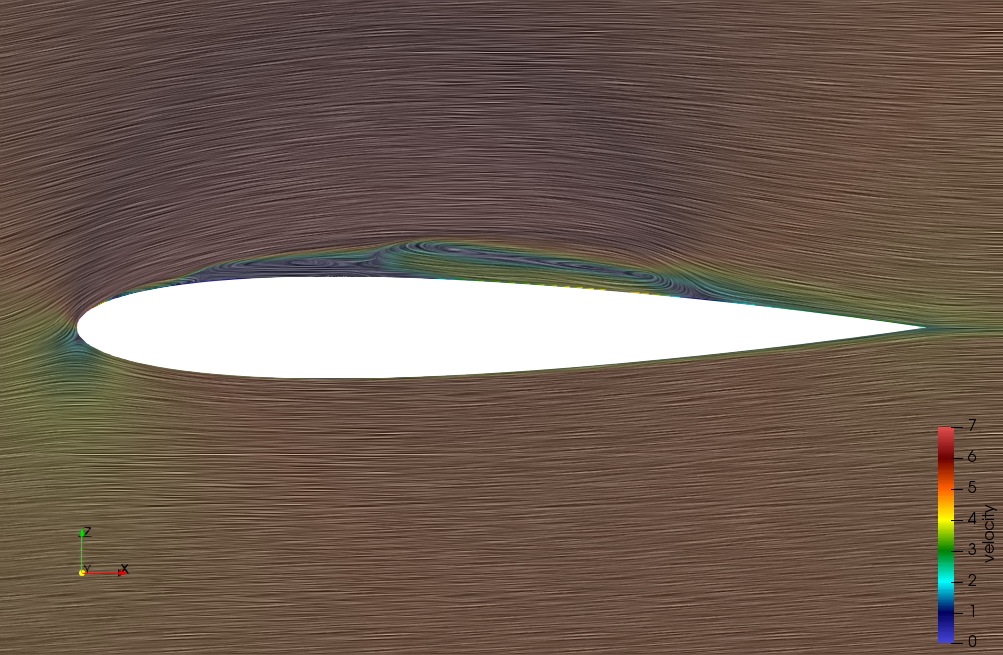
\includegraphics[width=0.3\textwidth]{AOA5.7p/AOA5.7t0.7RE}}} 
& \multicolumn{1}{l|}{\subfloat[t=0.8 s]{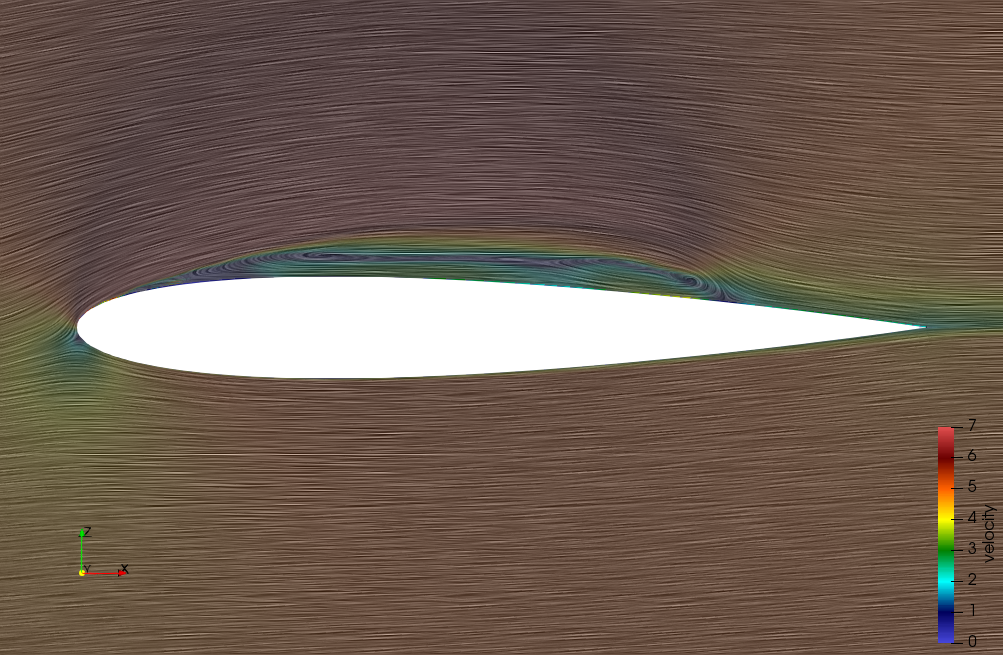
\includegraphics[width=0.3\textwidth]{AOA5.7p/AOA5.7t0.8RE}}} &\subfloat[t=1 s]{\includegraphics[width=0.3\textwidth]{AOA5.7p/AOA5.7t1RE}}  \\ \hline

\multicolumn{1}{|l|}{$\alpha={{6.5}^{\circ}}$} & \multicolumn{1}{l|}{\subfloat[t=0.8 s]{\includegraphics[width=0.3\textwidth]{AOA6.5p/AOA6.5t0.8RE}}} 
& \multicolumn{1}{l|}{\subfloat[t=0.9 s]{\includegraphics[width=0.3\textwidth]{AOA6.5p/AOA6.5t0.9RE}}} &\subfloat[t=1 s]{\includegraphics[width=0.3\textwidth]{AOA6.5p/AOA6.5t1RE}}  \\ \hline

\end{tabular}
\end{figure}
\end{table}  
 
 \begin{table}[h]
\centering
 \begin{figure}[H]
\begin{tabular}{|llll|} 
\hline
\rowcolor{gray!20} \multicolumn{4}{|l|}{Re-entrant at different angles of attack}\\ \hline
 \multicolumn{1}{|l|}{$\alpha={{7.6}^{\circ}}$} & \multicolumn{1}{l|}{\subfloat[t=0.6 s]{\includegraphics[width=0.3\textwidth]{AOA7.6p/AOA7.6t0.6RE}}} 
& \multicolumn{1}{l|}{\subfloat[t=0.82 s]{\includegraphics[width=0.3\textwidth]{AOA7.6p/AOA7.6t0.82RE}}} &\subfloat[t=0.92 s]{\includegraphics[width=0.3\textwidth]{AOA7.6p/AOA7.6t0.92RE}}  \\ \hline


  \multicolumn{1}{|l|}{$\alpha={{8}^{\circ}}$} & \multicolumn{1}{l|}{\subfloat[t=0.5 s]{\includegraphics[width=0.3\textwidth]{AOA8p/AOA8t0.5RE}}} 
& \multicolumn{1}{l|}{\subfloat[t=0.7 s]{\includegraphics[width=0.3\textwidth]{AOA8p/AOA8t0.7RE}}} &\subfloat[t=0.9 s]{\includegraphics[width=0.3\textwidth]{AOA8p/AOA8t0.9RE}}  \\ \hline
\end{tabular}
\end{figure}
\caption{Re-entrant jet over a NACA0012 hydrofoil at different angles of attack and time period}
 \label{fig:fig16}
\end{table} 
 
 \begin{table}[h]
\centering
 \begin{figure}[H]
\begin{tabular}{|llll|}
\hline
\rowcolor{gray!20} \multicolumn{4}{|l|}{alpha.water distribution for a different angles of attack}\\ \hline
\multicolumn{1}{|l|}{$\alpha={{4.1}^{\circ}}$} & \multicolumn{1}{l|}{\subfloat[t=0.6 s]{\includegraphics[width=0.3\textwidth]{AOA4.1p/AOA4.1t0.6alpha}}} 
& \multicolumn{1}{l|}{\subfloat[t=0.8 s]{\includegraphics[width=0.3\textwidth]{AOA4.1p/AOA4.1t0.8alpha}}} &\subfloat[t=1 s]{\includegraphics[width=0.3\textwidth]{AOA4.1p/AOA4.1t1alpha}}  \\ \hline

\multicolumn{1}{|l|}{$\alpha={{4.5}^{\circ}}$} & \multicolumn{1}{l|}{\subfloat[t=0.42 s]{\includegraphics[width=0.3\textwidth]{AOA4.5p/AOA4.5t0.42alpha}}} 
& \multicolumn{1}{l|}{\subfloat[t=0.66 s]{\includegraphics[width=0.3\textwidth]{AOA4.5p/AOA4.5t0.66alpha}}} & {\subfloat[t=0.72 s]{\includegraphics[width=0.3\textwidth]{AOA4.5p/AOA4.5t0.72alpha}}} \\ \hline

\multicolumn{1}{|l|}{$\alpha={{5.0}^{\circ}}$} & \multicolumn{1}{l|}{\subfloat[t=0.5 s]{\includegraphics[width=0.3\textwidth]{AOA5p/AOA5.0t0.5alpha}}} 
& \multicolumn{1}{l|}{\subfloat[t=0.7 s]{\includegraphics[width=0.3\textwidth]{AOA5p/AOA5.0t0.7alpha}}} &\subfloat[t=0.88 s]{\includegraphics[width=0.3\textwidth]{AOA5p/AOA5.0t0.88alpha}}  \\ \hline

\multicolumn{1}{|l|}{$\alpha={{5.7}^{\circ}}$} & \multicolumn{1}{l|}{\subfloat[t=0.7 s]{\includegraphics[width=0.3\textwidth]{AOA5.7p/AOA5.7t0.7alpha}}} 
& \multicolumn{1}{l|}{\subfloat[t=0.8 s]{\includegraphics[width=0.3\textwidth]{AOA5.7p/AOA5.7t0.8alpha}}} &\subfloat[t=1 s]{\includegraphics[width=0.3\textwidth]{AOA5.7p/AOA5.7t1alpha}}  \\ \hline

\multicolumn{1}{|l|}{$\alpha={{6.5}^{\circ}}$} & \multicolumn{1}{l|}{\subfloat[t=0.8 s]{\includegraphics[width=0.3\textwidth]{AOA6.5p/AOA6.5t0.8alpha}}} 
& \multicolumn{1}{l|}{\subfloat[t=0.9 s]{\includegraphics[width=0.3\textwidth]{AOA6.5p/AOA6.5t0.9alpha}}} &\subfloat[t=1 s]{\includegraphics[width=0.3\textwidth]{AOA6.5p/AOA6.5t1alpha}}  \\ \hline

\end{tabular}
\end{figure}
\end{table}  
 \begin{table}[h]
\centering
 \begin{figure}[H]
\begin{tabular}{|llll|} 
\hline
\rowcolor{gray!20} \multicolumn{4}{|l|}{alpha.water distribution for a different angles of attack}\\ \hline
 \multicolumn{1}{|l|}{$\alpha={{7.6}^{\circ}}$} & \multicolumn{1}{l|}{\subfloat[t=0.6 s]{\includegraphics[width=0.3\textwidth]{AOA7.6p/AOA7.6t0.6alpha}}} 
& \multicolumn{1}{l|}{\subfloat[t=0.82 s]{\includegraphics[width=0.3\textwidth]{AOA7.6p/AOA7.6t0.82alpha}}} &\subfloat[t=0.92 s]{\includegraphics[width=0.3\textwidth]{AOA7.6p/AOA7.6t0.92alpha}}  \\ \hline


  \multicolumn{1}{|l|}{$\alpha={{8}^{\circ}}$} & \multicolumn{1}{l|}{\subfloat[t=0.5 s]{\includegraphics[width=0.3\textwidth]{AOA8p/AOA8t0.5alpha}}} 
& \multicolumn{1}{l|}{\subfloat[t=0.7 s]{\includegraphics[width=0.3\textwidth]{AOA8p/AOA8t0.7alpha}}} &\subfloat[t=0.9 s]{\includegraphics[width=0.3\textwidth]{AOA8p/AOA8t0.9alpha}}  \\ \hline
\end{tabular}
\end{figure}
\caption{alpha.water distribution over a NACA0012 hydrofoil at different angles of attack and time period}
 \label{fig:fig16}
\end{table} 
 
 

\begin{table}[h]
\centering
 \begin{figure}[H]
\begin{tabular}{|llll|}
\hline
\rowcolor{gray!20} \multicolumn{4}{|l|}{Pressure distribution for a different angles of attack}\\ \hline
\multicolumn{1}{|l|}{$\alpha={{4.1}^{\circ}}$} & \multicolumn{1}{l|}{\subfloat[t=0.6 s]{\includegraphics[width=0.3\textwidth]{AOA4.1p/AOA4.1t0.6p}}} 
& \multicolumn{1}{l|}{\subfloat[t=0.8 s]{\includegraphics[width=0.3\textwidth]{AOA4.1p/AOA4.1t0.8p}}} &\subfloat[t=1 s]{\includegraphics[width=0.3\textwidth]{AOA4.1p/AOA4.1t1p}}  \\ \hline

\multicolumn{1}{|l|}{$\alpha={{4.5}^{\circ}}$} & \multicolumn{1}{l|}{\subfloat[t=0.42 s]{\includegraphics[width=0.3\textwidth]{AOA4.5p/AOA4.5t0.42p}}} 
& \multicolumn{1}{l|}{\subfloat[t=0.66 s]{\includegraphics[width=0.3\textwidth]{AOA4.5p/AOA4.5t0.66p}}} & {\subfloat[t=0.72 s]{\includegraphics[width=0.3\textwidth]{AOA4.5p/AOA4.5t0.72p}}} \\ \hline

\multicolumn{1}{|l|}{$\alpha={{5.0}^{\circ}}$} & \multicolumn{1}{l|}{\subfloat[t=0.5 s]{\includegraphics[width=0.3\textwidth]{AOA5p/AOA5.0t0.5p}}} 
& \multicolumn{1}{l|}{\subfloat[t=0.7 s]{\includegraphics[width=0.3\textwidth]{AOA5p/AOA5.0t0.7p}}} &\subfloat[t=0.88 s]{\includegraphics[width=0.3\textwidth]{AOA5p/AOA5.0t0.88p}}  \\ \hline

\multicolumn{1}{|l|}{$\alpha={{5.7}^{\circ}}$} & \multicolumn{1}{l|}{\subfloat[t=0.7 s]{\includegraphics[width=0.3\textwidth]{AOA5.7p/AOA5.7t0.7p}}} 
& \multicolumn{1}{l|}{\subfloat[t=0.8 s]{\includegraphics[width=0.3\textwidth]{AOA5.7p/AOA5.7t0.8p}}} &\subfloat[t=1 s]{\includegraphics[width=0.3\textwidth]{AOA5.7p/AOA5.7t1p}}  \\ \hline

\multicolumn{1}{|l|}{$\alpha={{6.5}^{\circ}}$} & \multicolumn{1}{l|}{\subfloat[t=0.8 s]{\includegraphics[width=0.3\textwidth]{AOA6.5p/AOA6.5t0.8p}}} 
& \multicolumn{1}{l|}{\subfloat[t=0.9 s]{\includegraphics[width=0.3\textwidth]{AOA6.5p/AOA6.5t0.9p}}} &\subfloat[t=1 s]{\includegraphics[width=0.3\textwidth]{AOA6.5p/AOA6.5t1p}}  \\ \hline

\end{tabular}
\end{figure}
\end{table}  
  
\begin{table}[h]
\centering
 \begin{figure}[H]
\begin{tabular}{|llll|} 
\hline
\rowcolor{gray!20} \multicolumn{4}{|l|}{Pressure distribution for a different angles of attack}\\ \hline
 \multicolumn{1}{|l|}{$\alpha={{7.6}^{\circ}}$} & \multicolumn{1}{l|}{\subfloat[t=0.6 s]{\includegraphics[width=0.3\textwidth]{AOA7.6p/AOA7.6t0.6p}}} 
& \multicolumn{1}{l|}{\subfloat[t=0.82 s]{\includegraphics[width=0.3\textwidth]{AOA7.6p/AOA7.6t0.82p}}} &\subfloat[t=0.92 s]{\includegraphics[width=0.3\textwidth]{AOA7.6p/AOA7.6t0.92p}}  \\ \hline


  \multicolumn{1}{|l|}{$\alpha={{8}^{\circ}}$} & \multicolumn{1}{l|}{\subfloat[t=0.5 s]{\includegraphics[width=0.3\textwidth]{AOA8p/AOA8t0.5p}}} 
& \multicolumn{1}{l|}{\subfloat[t=0.7 s]{\includegraphics[width=0.3\textwidth]{AOA8p/AOA8t0.7p}}} &\subfloat[t=0.9 s]{\includegraphics[width=0.3\textwidth]{AOA8p/AOA8t0.9p}}  \\ \hline
\end{tabular}
\end{figure}
\caption{Pressure distribution over a NACA0012 hydrofoil at different angles of attack and time period}
 \label{fig:fig16}
\end{table}


 
 \begin{table}[h]
\centering
 \begin{figure}[H]
\begin{tabular}{|llll|}
\hline
\rowcolor{gray!20} \multicolumn{4}{|l|}{$C_p$ distribution for a different angles of attack}\\ \hline
\multicolumn{1}{|l|}{$\alpha={{4.1}^{\circ}}$} & \multicolumn{1}{l|}{\subfloat[t=0.6 s]{\includegraphics[width=0.3\textwidth]{AOA4.1p/AOA4.1t0.6cp}}} 
& \multicolumn{1}{l|}{\subfloat[t=0.8 s]{\includegraphics[width=0.3\textwidth]{AOA4.1p/AOA4.1t0.8cp}}} &\subfloat[t=1 s]{\includegraphics[width=0.3\textwidth]{AOA4.1p/AOA4.1t1cp}}  \\ \hline

\multicolumn{1}{|l|}{$\alpha={{4.5}^{\circ}}$} & \multicolumn{1}{l|}{\subfloat[t=0.42 s]{\includegraphics[width=0.3\textwidth]{AOA4.5p/AOA4.5t0.42cp}}} 
& \multicolumn{1}{l|}{\subfloat[t=0.66 s]{\includegraphics[width=0.3\textwidth]{AOA4.5p/AOA4.5t0.66cp}}} & {\subfloat[t=0.72 s]{\includegraphics[width=0.3\textwidth]{AOA4.5p/AOA4.5t0.72cp}}} \\ \hline

\multicolumn{1}{|l|}{$\alpha={{5.0}^{\circ}}$} & \multicolumn{1}{l|}{\subfloat[t=0.5 s]{\includegraphics[width=0.3\textwidth]{AOA5p/AOA5.0t0.5cp}}} 
& \multicolumn{1}{l|}{\subfloat[t=0.7 s]{\includegraphics[width=0.3\textwidth]{AOA5p/AOA5.0t0.7cp}}} &\subfloat[t=0.88 s]{\includegraphics[width=0.3\textwidth]{AOA5p/AOA5.0t0.88cp}}  \\ \hline

\multicolumn{1}{|l|}{$\alpha={{5.7}^{\circ}}$} & \multicolumn{1}{l|}{\subfloat[t=0.7 s]{\includegraphics[width=0.3\textwidth]{AOA5.7p/AOA5.7t0.7cp}}} 
& \multicolumn{1}{l|}{\subfloat[t=0.8 s]{\includegraphics[width=0.3\textwidth]{AOA5.7p/AOA5.7t0.8cp}}} &\subfloat[t=1 s]{\includegraphics[width=0.3\textwidth]{AOA5.7p/AOA5.7t1cp}}  \\ \hline

\multicolumn{1}{|l|}{$\alpha={{6.5}^{\circ}}$} & \multicolumn{1}{l|}{\subfloat[t=0.8 s]{\includegraphics[width=0.3\textwidth]{AOA6.5p/AOA6.5t0.8cp}}} 
& \multicolumn{1}{l|}{\subfloat[t=0.9 s]{\includegraphics[width=0.3\textwidth]{AOA6.5p/AOA6.5t0.9cp}}} &\subfloat[t=1 s]{\includegraphics[width=0.3\textwidth]{AOA6.5p/AOA6.5t1cp}}  \\ \hline

\end{tabular}
\end{figure}
\end{table}  
 \begin{table}[h]
\centering
 \begin{figure}[H]
\begin{tabular}{|llll|} 
\hline
\rowcolor{gray!20} \multicolumn{4}{|l|}{$C_p$ distribution for a different angles of attack}\\ \hline
 \multicolumn{1}{|l|}{$\alpha={{7.6}^{\circ}}$} & \multicolumn{1}{l|}{\subfloat[t=0.6 s]{\includegraphics[width=0.3\textwidth]{AOA7.6p/AOA7.6t0.6cp}}} 
& \multicolumn{1}{l|}{\subfloat[t=0.82 s]{\includegraphics[width=0.3\textwidth]{AOA7.6p/AOA7.6t0.82cp}}} &\subfloat[t=0.92 s]{\includegraphics[width=0.3\textwidth]{AOA7.6p/AOA7.6t0.92cp}}  \\ \hline


  \multicolumn{1}{|l|}{$\alpha={{8}^{\circ}}$} & \multicolumn{1}{l|}{\subfloat[t=0.5 s]{\includegraphics[width=0.3\textwidth]{AOA8p/AOA8t0.5cp}}} 
& \multicolumn{1}{l|}{\subfloat[t=0.7 s]{\includegraphics[width=0.3\textwidth]{AOA8p/AOA8t0.7cp}}} &\subfloat[t=0.9 s]{\includegraphics[width=0.3\textwidth]{AOA8p/AOA8t0.9cp}}  \\ \hline
\end{tabular}
\end{figure}
\caption{$C_p$ distribution over a NACA0012 hydrofoil at different angles of attack and time period}
 \label{fig:fig16}
\end{table} 
 
 

 
 \begin{table}[h]
\centering
 \begin{figure}[H]
\begin{tabular}{|llll|}
\hline
\rowcolor{gray!20} \multicolumn{4}{|l|}{$C_p$ vs x/c}\\ \hline
\multicolumn{1}{|l|}{$\alpha={{4.1}^{\circ}}$} & \multicolumn{1}{l|}{\subfloat[t=0.6 s]{\includegraphics[width=0.3\textwidth]{thesisgraph/AOA4.1t0.6cp}}} 
& \multicolumn{1}{l|}{\subfloat[t=0.8 s]{\includegraphics[width=0.3\textwidth]{thesisgraph/AOA4.1t0.8cp}}} &\subfloat[t=1 s]{\includegraphics[width=0.3\textwidth]{thesisgraph/AOA4.1t1cp}}  \\ \hline

\multicolumn{1}{|l|}{$\alpha={{4.5}^{\circ}}$} & \multicolumn{1}{l|}{\subfloat[t=0.42 s]{\includegraphics[width=0.3\textwidth]{thesisgraph/AOA4.5t0.42cp}}} 
& \multicolumn{1}{l|}{\subfloat[t=0.66 s]{\includegraphics[width=0.3\textwidth]{thesisgraph/AOA4.5t0.66cp}}} & {\subfloat[t=0.72 s]{\includegraphics[width=0.3\textwidth]{thesisgraph/AOA4.5t0.72cp}}} \\ \hline

\multicolumn{1}{|l|}{$\alpha={{5.0}^{\circ}}$} & \multicolumn{1}{l|}{\subfloat[t=0.5 s]{\includegraphics[width=0.3\textwidth]{thesisgraph/AOA5.09t0.5cp}}} 
& \multicolumn{1}{l|}{\subfloat[t=0.7 s]{\includegraphics[width=0.3\textwidth]{thesisgraph/AOA5.09t0.7cp}}} &\subfloat[t=0.88 s]{\includegraphics[width=0.3\textwidth]{thesisgraph/AOA5.09t0.88cp}}  \\ \hline

\multicolumn{1}{|l|}{$\alpha={{5.7}^{\circ}}$} & \multicolumn{1}{l|}{\subfloat[t=0.7 s]{\includegraphics[width=0.3\textwidth]{thesisgraph/AOA5.7t0.7cp}}} 
& \multicolumn{1}{l|}{\subfloat[t=0.8 s]{\includegraphics[width=0.3\textwidth]{thesisgraph/AOA5.7t0.8cp}}} &\subfloat[t=1 s]{\includegraphics[width=0.3\textwidth]{thesisgraph/AOA5.7t1cp}}  \\ \hline
\end{tabular}
\end{figure}
\end{table}  

 
 \begin{table}[h]
\centering
 \begin{figure}[H]
\begin{tabular}{|llll|} 
\hline
\rowcolor{gray!20} \multicolumn{4}{|l|}{$C_p$ vs x/c}\\ \hline
\multicolumn{1}{|l|}{$\alpha={{6.5}^{\circ}}$} & \multicolumn{1}{l|}{\subfloat[t=0.8 s]{\includegraphics[width=0.3\textwidth]{thesisgraph/AOA6.5t0.8cp}}} 
& \multicolumn{1}{l|}{\subfloat[t=0.9 s]{\includegraphics[width=0.3\textwidth]{thesisgraph/AOA6.5t0.9cp}}} &\subfloat[t=1 s]{\includegraphics[width=0.3\textwidth]{thesisgraph/AOA6.5t1cp}}  \\ \hline


 \multicolumn{1}{|l|}{$\alpha={{7.6}^{\circ}}$} & \multicolumn{1}{l|}{\subfloat[t=0.6 s]{\includegraphics[width=0.3\textwidth]{thesisgraph/AOA7.6t0.6cp}}} 
& \multicolumn{1}{l|}{\subfloat[t=0.82 s]{\includegraphics[width=0.3\textwidth]{thesisgraph/AOA7.6t0.82cp}}} &\subfloat[t=0.92 s]{\includegraphics[width=0.3\textwidth]{thesisgraph/AOA7.6t0.92cp}}  \\ \hline


  \multicolumn{1}{|l|}{$\alpha={{8}^{\circ}}$} & \multicolumn{1}{l|}{\subfloat[t=0.5 s]{\includegraphics[width=0.3\textwidth]{thesisgraph/AOA8t0.5cp}}} 
& \multicolumn{1}{l|}{\subfloat[t=0.7 s]{\includegraphics[width=0.3\textwidth]{thesisgraph/AOA8t0.7cp}}} &\subfloat[t=0.9 s]{\includegraphics[width=0.3\textwidth]{thesisgraph/AOA8t0.9cp}}  \\ \hline
\end{tabular}
\end{figure}
\caption{$C_p$ vs x/c graph for different angles of attack and time period}
 \label{fig:fig16}
\end{table} 
  
 \begin{table}[h]
 \centering
 \begin{figure}[H]
\begin{tabular}{|lll|}
\hline
\rowcolor{gray!20}\multicolumn{3}{|l|}{Force coefficient and statistical average at different angles attack} \\ \hline
\multicolumn{1}{|l|}{$\alpha={{4.1}^{\circ}}$} & \multicolumn{1}{l|}{\subfloat[]{\includegraphics[width=0.3\textwidth]{thesisgraph/AOA4.1cl}}} & 
{\subfloat[]{\includegraphics[width=0.3\textwidth]{thesisgraph/AOA4.1cd}}} \\ \hline

\multicolumn{1}{|l|}{$\alpha={{4.5}^{\circ}}$} & \multicolumn{1}{l|}{\subfloat[]{\includegraphics[width=0.3\textwidth]{thesisgraph/AOA4.5cl}}} 
& {\subfloat[]{\includegraphics[width=0.3\textwidth]{thesisgraph/AOA4.5cd}}} \\ \hline

\multicolumn{1}{|l|}{$\alpha={{5.0}^{\circ}}$} & \multicolumn{1}{l|}{\subfloat[]{\includegraphics[width=0.3\textwidth]{thesisgraph/AOA5.09cl}}} 
& {\subfloat[]{\includegraphics[width=0.3\textwidth]{thesisgraph/AOA5.09cd}}} \\ \hline

\multicolumn{1}{|l|}{$\alpha={{5.7}^{\circ}}$} & \multicolumn{1}{l|}{\subfloat[]{\includegraphics[width=0.3\textwidth]{thesisgraph/AOA5.7cl}}} 
& {\subfloat[]{\includegraphics[width=0.3\textwidth]{thesisgraph/AOA5.7cd}}} \\ \hline


\end{tabular}
\end{figure}
\end{table}
 
 \begin{table}[h]
 \centering
 \begin{figure}[H]
\begin{tabular}{|lll|}
\hline
\rowcolor{gray!20}\multicolumn{3}{|l|}{Force coefficient and statistical average at different angles attack} \\ \hline
\multicolumn{1}{|l|}{$\alpha={{6.5}^{\circ}}$} & \multicolumn{1}{l|}{\subfloat[]{\includegraphics[width=0.3\textwidth]{thesisgraph/AOA6.5cl}}} & 
{\subfloat[]{\includegraphics[width=0.3\textwidth]{thesisgraph/AOA6.5cd}}} \\ \hline

\multicolumn{1}{|l|}{$\alpha={{7.6}^{\circ}}$} & \multicolumn{1}{l|}{\subfloat[]{\includegraphics[width=0.3\textwidth]{thesisgraph/AOA7.6cl}}} 
& {\subfloat[]{\includegraphics[width=0.3\textwidth]{thesisgraph/AOA7.6cd}}} \\ \hline

\multicolumn{1}{|l|}{$\alpha={{8}^{\circ}}$} & \multicolumn{1}{l|}{\subfloat[]{\includegraphics[width=0.3\textwidth]{thesisgraph/AOA8cl}}} 
& {\subfloat[]{\includegraphics[width=0.3\textwidth]{thesisgraph/AOA8cd}}} \\ \hline
\end{tabular}
\end{figure}
\caption{Force coefficient at different angles of attack over a NACA0012}
\label{fig:fig16}
\end{table}
 
 
 
 
 
 
 
 
 
 
 
 
 
 
  
  
